\section{Facit}

\setcounter{opgave}{0}

\subsection*{Elektrostatik}

\begin{opgave}{Coulombkraften}
    \opg Indsættes de opgivne tal fås
    \begin{enumerate}
        \item $F = \dfrac{1}{4\pi\epsilon_0}\dfrac{q_1q_2}{r^2} = \SI{8.99e9}{\newton} = \SI{8.99}{\giga\newton}$.
        \item $F = \dfrac{1}{4\pi\epsilon_0}\dfrac{q_1q_2}{r^2} = -\SI{8.99e9}{\newton} = -\SI{8.99}{\giga\newton}$.
        \item $F = \dfrac{1}{4\pi\epsilon_0}\dfrac{q_1q_2}{r^2} = \SI{18.0e9}{\newton} = \SI{18.0}{\giga\newton}$.
        \item $F = \dfrac{1}{4\pi\epsilon_0}\dfrac{q_1q_2}{r^2} = \SI{2.25e9}{\newton} = \SI{2.25}{\giga\newton}$.
    \end{enumerate}
    \[ \]
    \opg Når den ene ladning skifter fortegn, så skifter kraften også fortegn. Fordobles størrelsen af den ene ladning, så fordobles størrelsen af kraften.
    \[ q_1\to -2q_1 \]
    Derudover bliver ladningernes indbyrdes afstand fordoblet.
    \[ r\to 2r\]
    Så vi har at kraften bliver
    \[ F=\frac{1}{4\pi\varepsilon_0}\frac{q_1q_2}{r^2}\to\frac{1}{4\pi\varepsilon_0}\frac{(-2q_1)q_2}{(2r)^2}=-\frac{1}{2}F.\]
    Kraften bliver dermed halvt så stor og skifter retning.
    \opg Vi skal bruge tilfælde 1. fra delopgave 1).
    \[ F=\SI{8.99e9}{\newton} \]
    Her er $m_1=\SI{1.00}{\kilo\gram}$ og $m_2=\SI{2.00}{\kilo\gram}$.
    Accelerationen på de to ladninger er
    \[ a_1 = \dfrac{F}{m_1} = \dfrac{1}{4\pi\epsilon_0}\dfrac{q_1q_2}{m_1r^2} = \SI{8.99e9}{\metre\per\second\squared} \]
    og
    \[ a_2 = \dfrac{F}{m_1} = \dfrac{1}{4\pi\epsilon_0}\dfrac{q_1q_2}{m_2r^2} = \SI{4.49e9}{\metre\per\second\squared}\]
    Her accelererer væk fra hinanden.
    \opg Her fås
    %
    \begin{enumerate}
        \setcounter{enumi}{1}
        \item $a_1 = \dfrac{F}{m_1} = \dfrac{1}{4\pi\epsilon_0}\dfrac{q_1q_2}{m_1r^2} = -\SI{8.99e9}{\metre\per\second\squared} = -\SI{8.99}{\giga\metre\per\second\squared}$.
        \item $a_1 = \dfrac{F}{m_1} = \dfrac{1}{4\pi\epsilon_0}\dfrac{q_1q_2}{m_1r^2} = \SI{18.0e9}{\metre\per\second\squared} = \SI{18.0}{\giga\metre\per\second\squared}$.
        \item $a_1 = \dfrac{F}{m_1} = \dfrac{1}{4\pi\epsilon_0}\dfrac{q_1q_2}{m_1r^2} = \SI{2.25e9}{\metre\per\second\squared} = \SI{2.25}{\giga\metre\per\second\squared}$.
    \end{enumerate}
    I 2. accelererer ladningerne mod hinanden, og væk fra hinanden i 3. og 4.
    \opg Da $m_2 = 2m_1$ accelereres ladning $1$ dobbelt så hurtigt som ladning $2$ uanset hvad kraften er. I tilfælde $1$, $3$ og $4$ har ladningerne samme fortegn, hvorfor de frastøder hinanden og dermed bevæger sig væk fra hinanden. Forskellen på tilfælde $1$ og $3$ er størrelsen på ladningen. Bevægelserne ser derfor ens ud, men alting går dobbelt så hurtigt i tilfælde $3$ som i tilfælde $1$. I tilfælde $4$ starter ladningerne dobbelt så langt fra hinanden som i tilfælde $1$. Selve bevægelsen vil stadig være ens, da det er den samme kraft i begge tilfælde. Alting vil dog gå $1/4$ så langsomt. I disse tre tilfælde vil ladningerne bevæge sig hurtigere og hurtigere væk fra hinanden og forsvinde uendeligt langt væk fra hinanden. Deres acceleration vil dog blive mindre og mindre. I tilfælde $2$ vil de to ladninger tiltrække hinanden, hvorfor de vil bevæge sig tættere og tættere på hinanden. Kraften på dem vil hele tiden øges, hvor accelerationen hele tid stiger. I et kort tidsrum efter de to ladninger frigives vil størrelserne på hastighederne i tilfælde $1$ og $2$ minde om hinanden, men dette holder op med at være tilfældet, når ladningernes indbyrdes afstand har ændret sig betydeligt fra udgangspunktet.
\end{opgave}

\begin{opgave}{Elektriske feltlinjer}
    \opg 
    \begin{figure}[H]
        \centering
        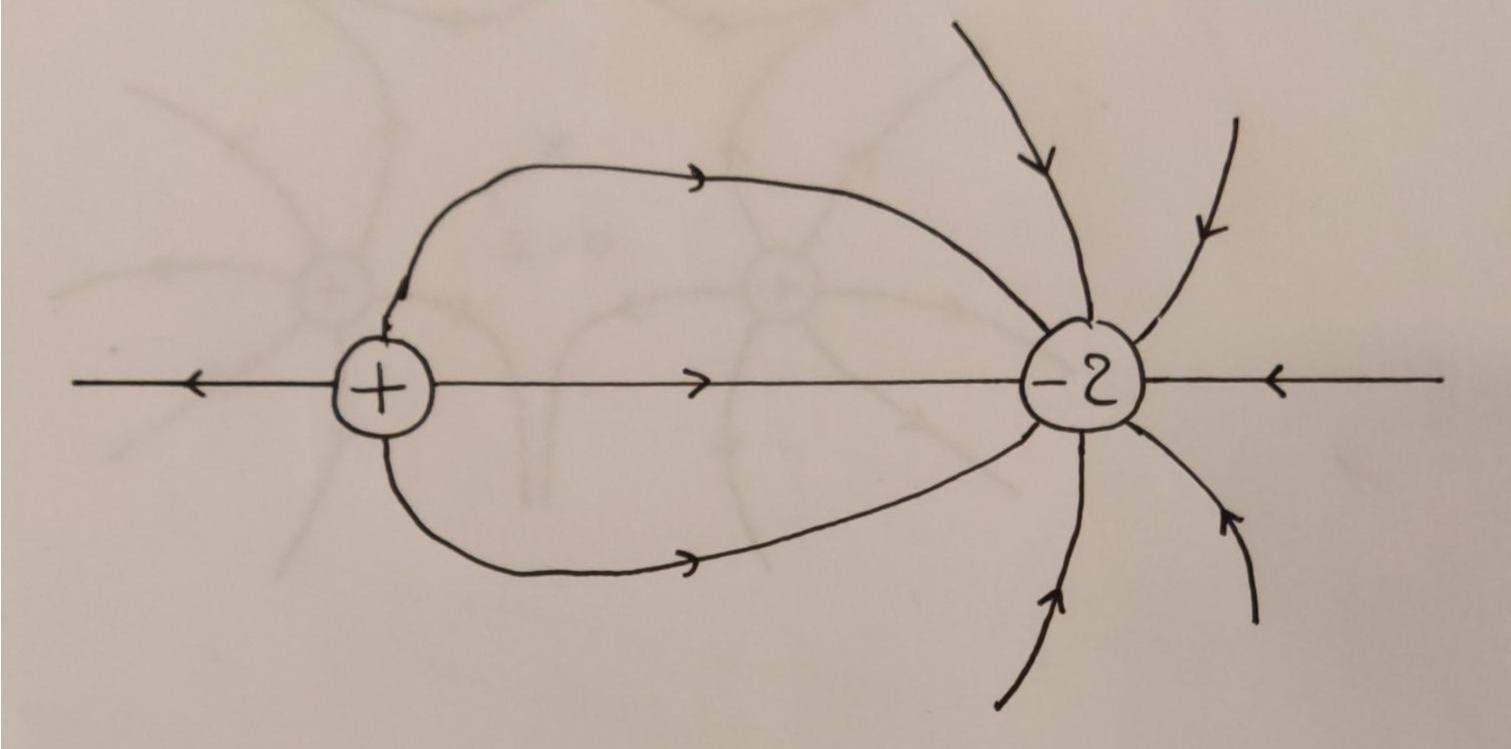
\includegraphics[width=0.8\textwidth]{facit/figurer/elektro/elektro_opg2,1.jpg}
    \end{figure}
    \opg
    \begin{figure}[H]
        \centering
        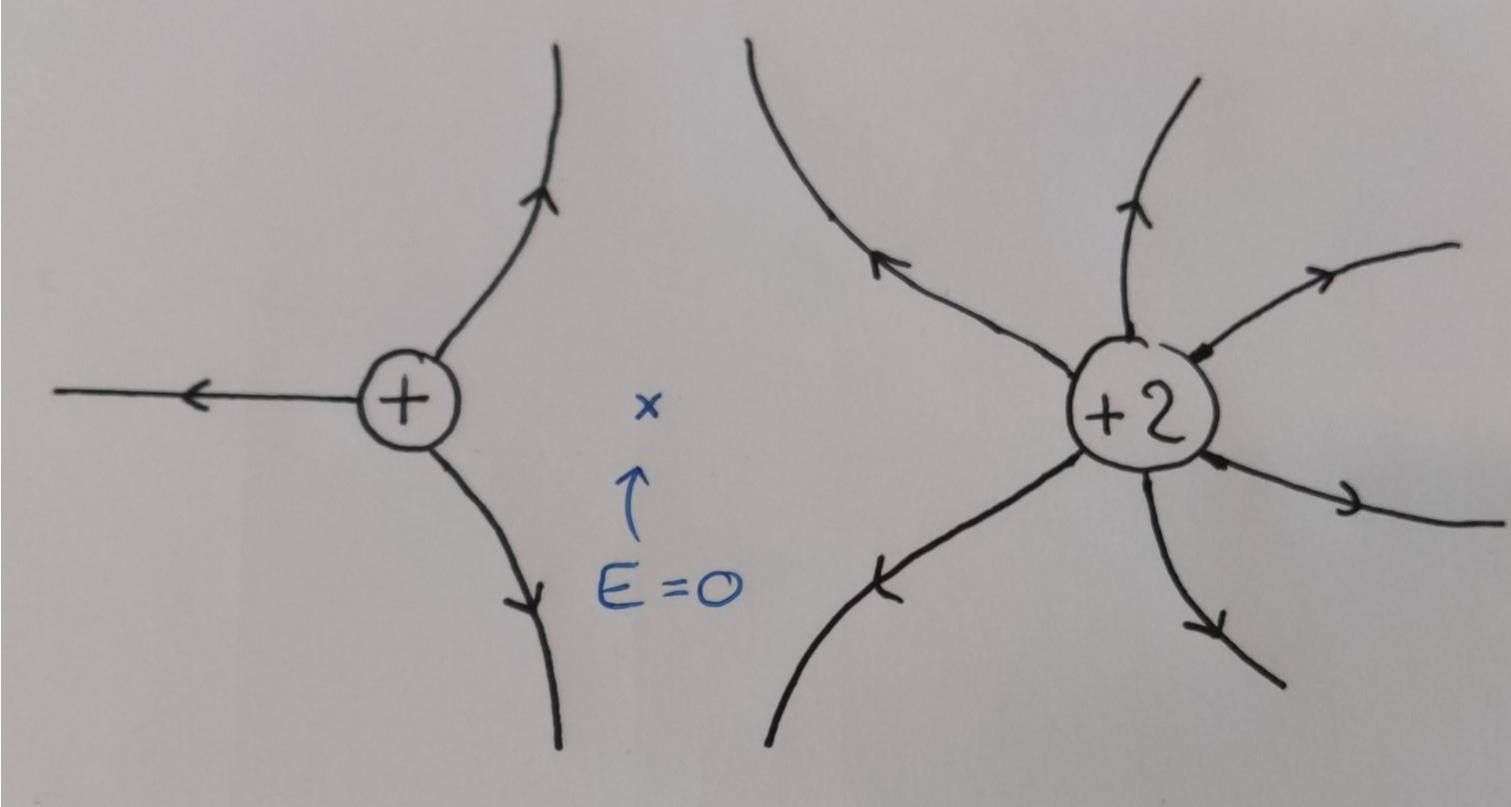
\includegraphics[width=0.8\textwidth]{facit/figurer/elektro/elektro_opg2,2.jpg}
    \end{figure}
    \opg 
    \begin{figure}[H]
        \centering
        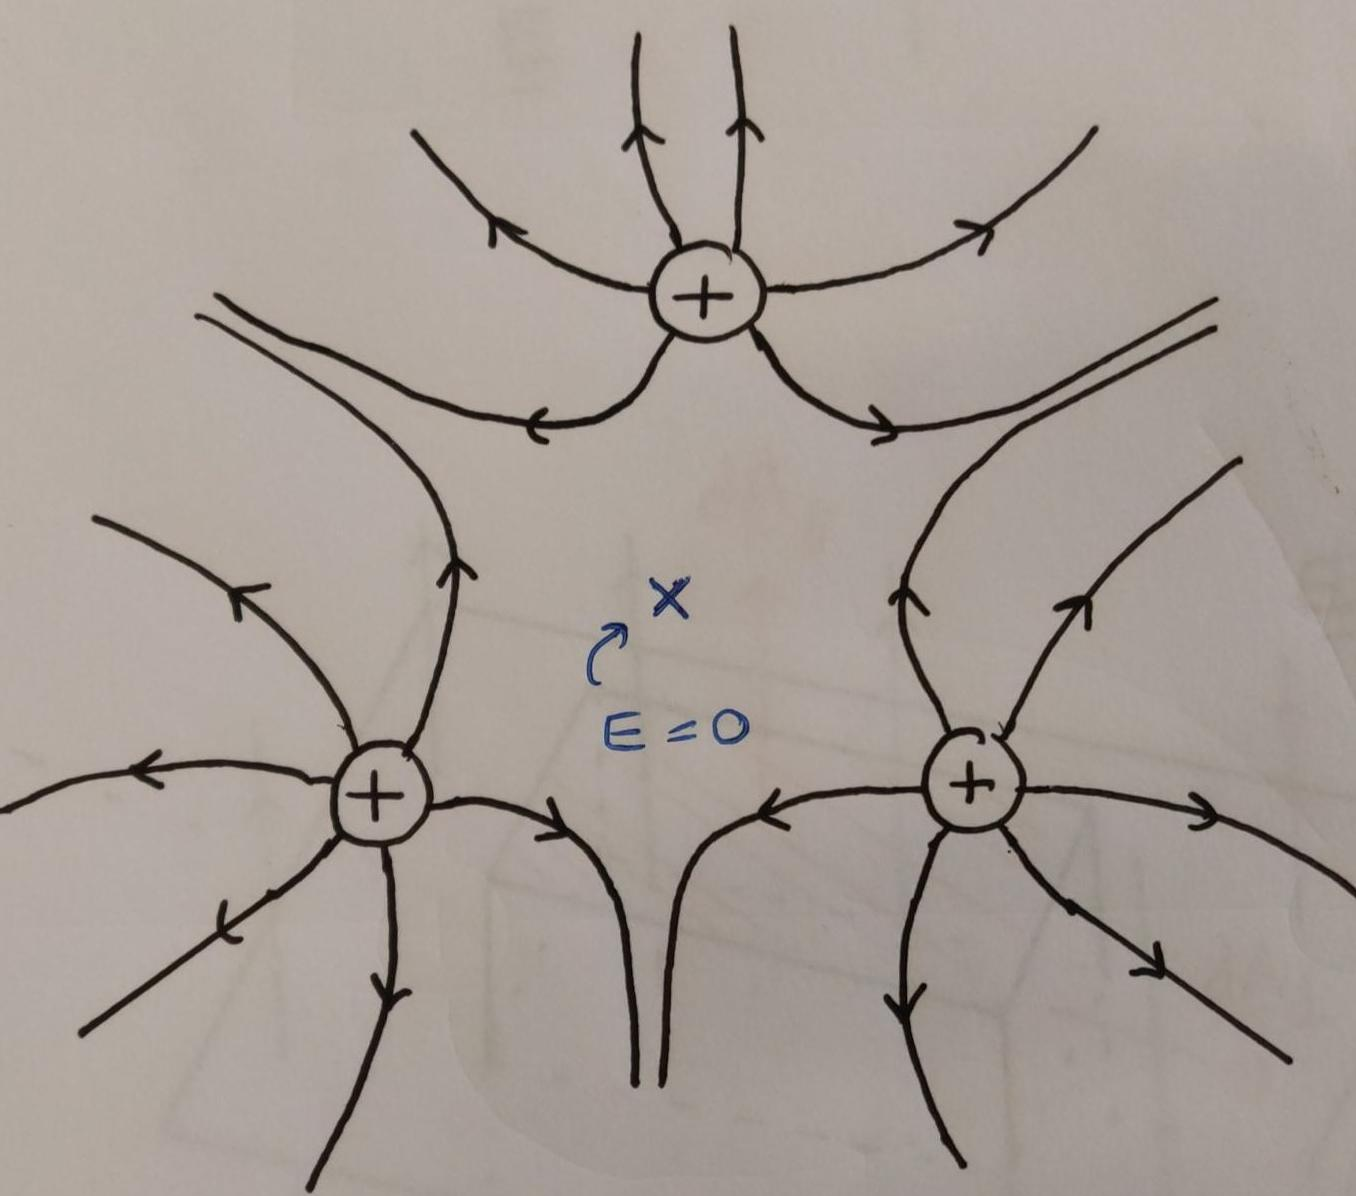
\includegraphics[width=0.8\textwidth]{facit/figurer/elektro/elektro_opg2,3.jpg}
    \end{figure}
\end{opgave}

\begin{opgave}{Tre ladninger på en linje}
    \opg Ved at bruge superpositionsprincippet, bliver dette
    \[ F=\frac{1}{4\pi\varepsilon_0}\left(\frac{Qq}{(x-a)^2}+\frac{Qq}{(x+a)^2}\right). \]
    \opg
    \begin{figure}[H]
        \centering
        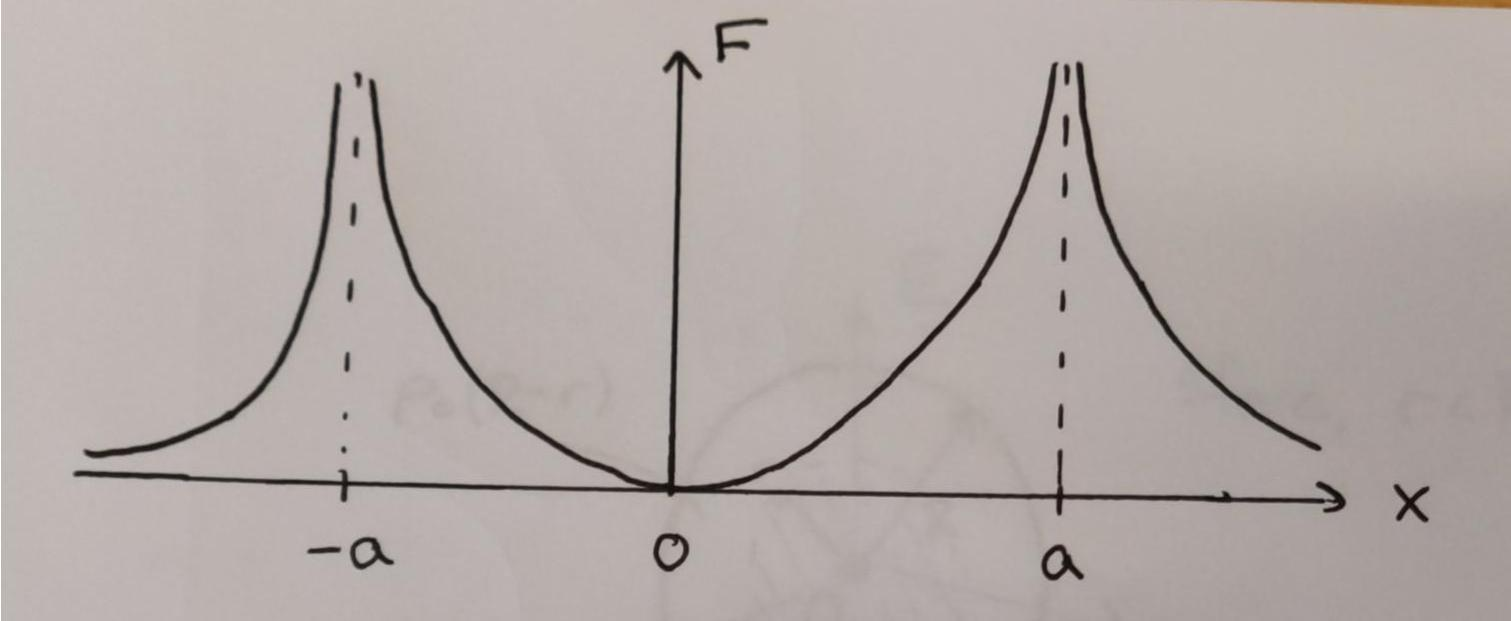
\includegraphics[width=0.8\textwidth]{facit/figurer/elektro/elektro_opg3,2.jpg}
    \end{figure}
    \opg Ved $x=0$ så er $F=0$, så ladningen $q$ står stille.
    \opg For $x\gg a$ bliver
    \begin{align*}
        F&=\frac{Qq}{4\pi\varepsilon_0}\left(\frac{1}{(x-a)^2}+\frac{1}{(x+a)^2}\right)\\
        &=\frac{Qq}{4\pi\varepsilon_0}\left(\frac{1}{\left(1-\cancelto{0}{\frac{a}{x}}\right)}+\frac{1}{\left(1+\cancelto{0}{\frac{a}{x}}\right)}\right)\frac{1}{x^2}\\
        &\approx \frac{Qq}{2\pi\varepsilon_0 x^2}\\
        &=\frac{1}{4\pi\varepsilon_0}\frac{(2Q)q}{x^2},
    \end{align*}
    hvilket er kraften på en ladning $q$ pga. en ladning $2Q$ placeret ved $x=0$. Når man er langt væk, kan man nemlig betragte begge $+Q$ ladninger som værende én samlet ladning.
\end{opgave}


\begin{opgave}{Bohrs atommodel}
    \opg Størrelsen af Coulombkraften på elektronen er $|F| = \dfrac{1}{4\pi\epsilon_0}\dfrac{e^2}{r^2} = \SI{8.24e-8}{\newton} = \SI{82.4}{\nano\newton}$.
    \opg Sættes centripetalkraften lig med Coulomkraften fås
    %
    \begin{align*}
        \frac{mv^2}{r} &= \frac{1}{4\pi\epsilon_0}\frac{e^2}{r^2}, \\
        \implies v &= \sqrt{\frac{1}{4\pi\epsilon_0}\frac{e^2}{mr}} = \SI{2.19e6}{\metre\per\second}.
    \end{align*}
    \opg $q(t)$ er en funktion, der beskriver ladningens mængden af ladning inde i området. Tætheden af ladning i bevægelse er $n = \SI{1}{\per\cubic\bohr}$, som bevæger sig i arealet $A = \pi\si{\bohr}^2$. $x(t)$ fortæller placeringen af ladningen og $-\si{\elementarycharge}$ er størrelsen på elektronens ladning. Ganges alle disse størrelser sammen fås en funktion med enheden ladning, der beskriver hvor meget ladning, der er i bevægelse omkring protonen, hvorfor $q(t) = -n\si{\elementarycharge}\pi\si{\bohr\squared}x(t)$ bruges.
    \opg Nu kan ligning \eqref{eq:current} bruges til at estimere strømstyrken en elektron generer i hydrogenatomet.
    %
    \begin{align*}
        I = \dv{q(t)}{t} = -n\si{\elementarycharge}\pi\si{\bohr\squared}\dv{x(t)}{t} = -n\si{\elementarycharge}\pi\si{\bohr\squared}v \approx \SI{20}{\milli\ampere}.
    \end{align*}
\end{opgave}

\begin{opgave}{Uendelig lang ladet linje}
    \opg
    \begin{figure}[H]
        \centering
        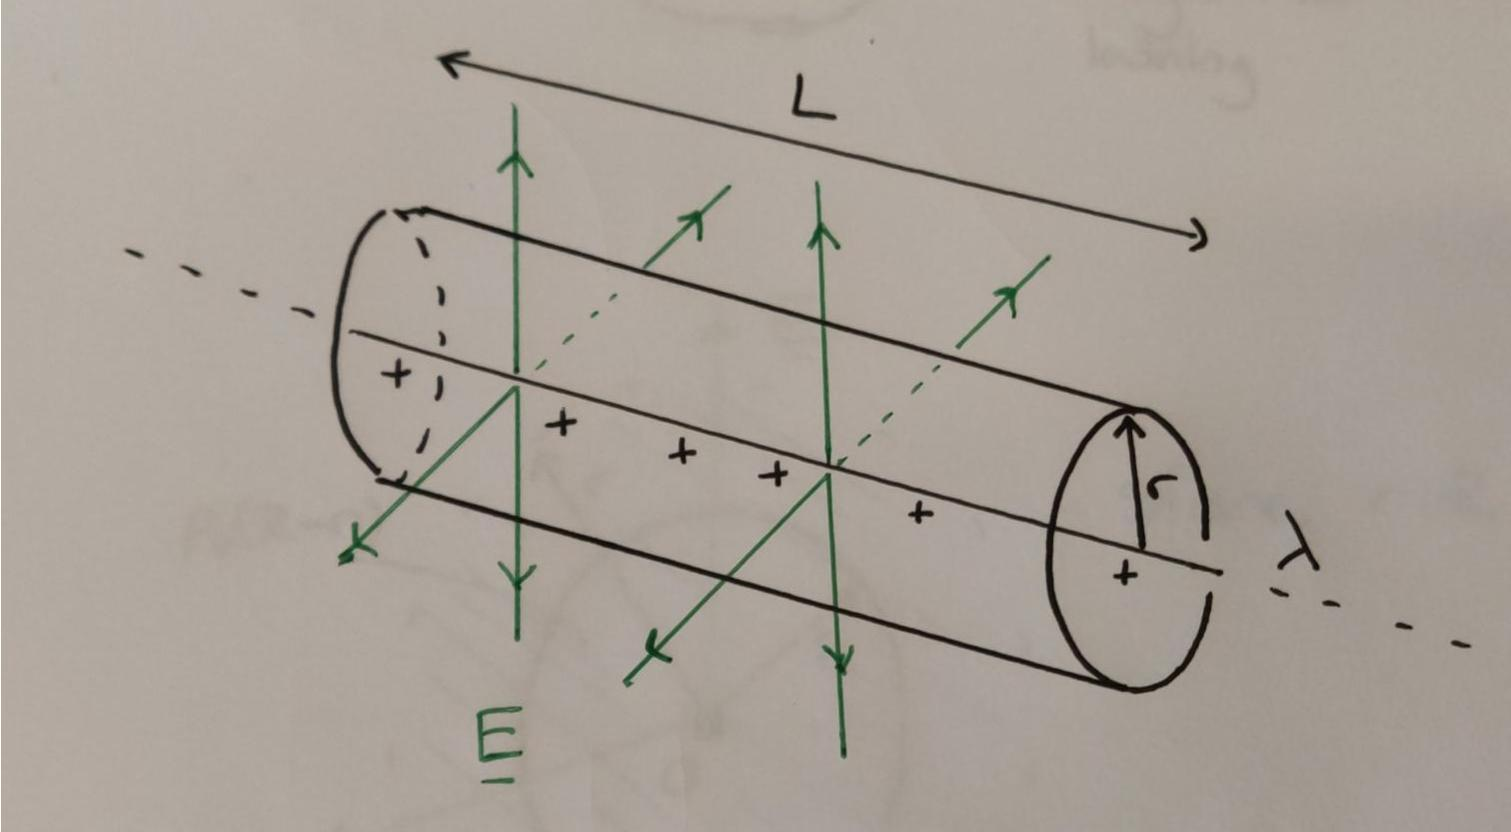
\includegraphics[width=0.8\textwidth]{facit/figurer/elektro/elektro_opg5,1.jpg}
    \end{figure}
    \opg Ladningen per længde er $\lambda$. I en $L$ lang cylinder er den samlede ladning derfor
    \[ Q_{inde}=\lambda L. \]
    \opg Reglerne for at tegne feltlinjer siger, at de ikke må røre hinanden. Den eneste retning en feltlinje kan udstrække sig, og fordi der er translatorisk symmetri langs linjen, er derfor væk fra linjen.
    \opg For endestykkerne peger det elektriske felt hen over overfladen, hvilket vil sige at den er vinkelret på arealvektoren. Så $\va E\cdot \dd\va A=0$.\\
    For den krumme overflade peger det elektriske felt vinkelret på overfladen, så $\va E$ og $\dd\va A$ må pege i samme retning. Så $\va E\cdot \dd\va A=E\dd A$.
    \opg Bruger vi ovenstående resultat, bliver integralet
    \begin{align*}
        \oint_S \va E \cdot \dd{\va A} &= \int_{S_1} \cancelto{E\dd A}{\va E \cdot \dd{\va A}} \enspace + \enspace \int_{S_2} \cancelto{0}{\va E \cdot \dd{\va A}} + \int_{S_3} \cancelto{0}{\va E \cdot \dd{\va A}}\\
        &=2\pi r L E
    \end{align*}
    siden $2\pi rL$ er arealet af den krumme overflade på et linjestykke med længde $L$.
    \opg Gauss' lov siger at
    \[ \oint_S \va E\cdot \dd \va A=\frac{Q_\text{inde}}{\varepsilon_0}. \]
    Sætter vi resultatet fra forrige opgave sammen med resultatet for ladningen i lederen, giver det
    \[ 2\pi rLE=\frac{\lambda L}{\varepsilon_0}. \]
    Løses for den elektriske feltstyrke som funktion af afstanden fra lederen, $E(r)$, fås
    \[ E(r)=\frac{\lambda}{2\pi\varepsilon_0 r}. \]
    Hvis vi skal skrive feltstyrken som en vektor, skal vi også kende dens retning. Hvis $\vu r$ er enhedsvektoren der peger væk fra linjen, må
    \[ \va E=E(r)\vu r =\frac{\lambda}{2\pi\varepsilon_0 r}\vu r.\]
    Bemærk, at vektorens størrelse bliver mindre, jo længere væk fra linjen du kommer.
\end{opgave}

\begin{opgave}{Uendeligt ladet plan}
    \opg
    \begin{figure}[H]
        \centering
        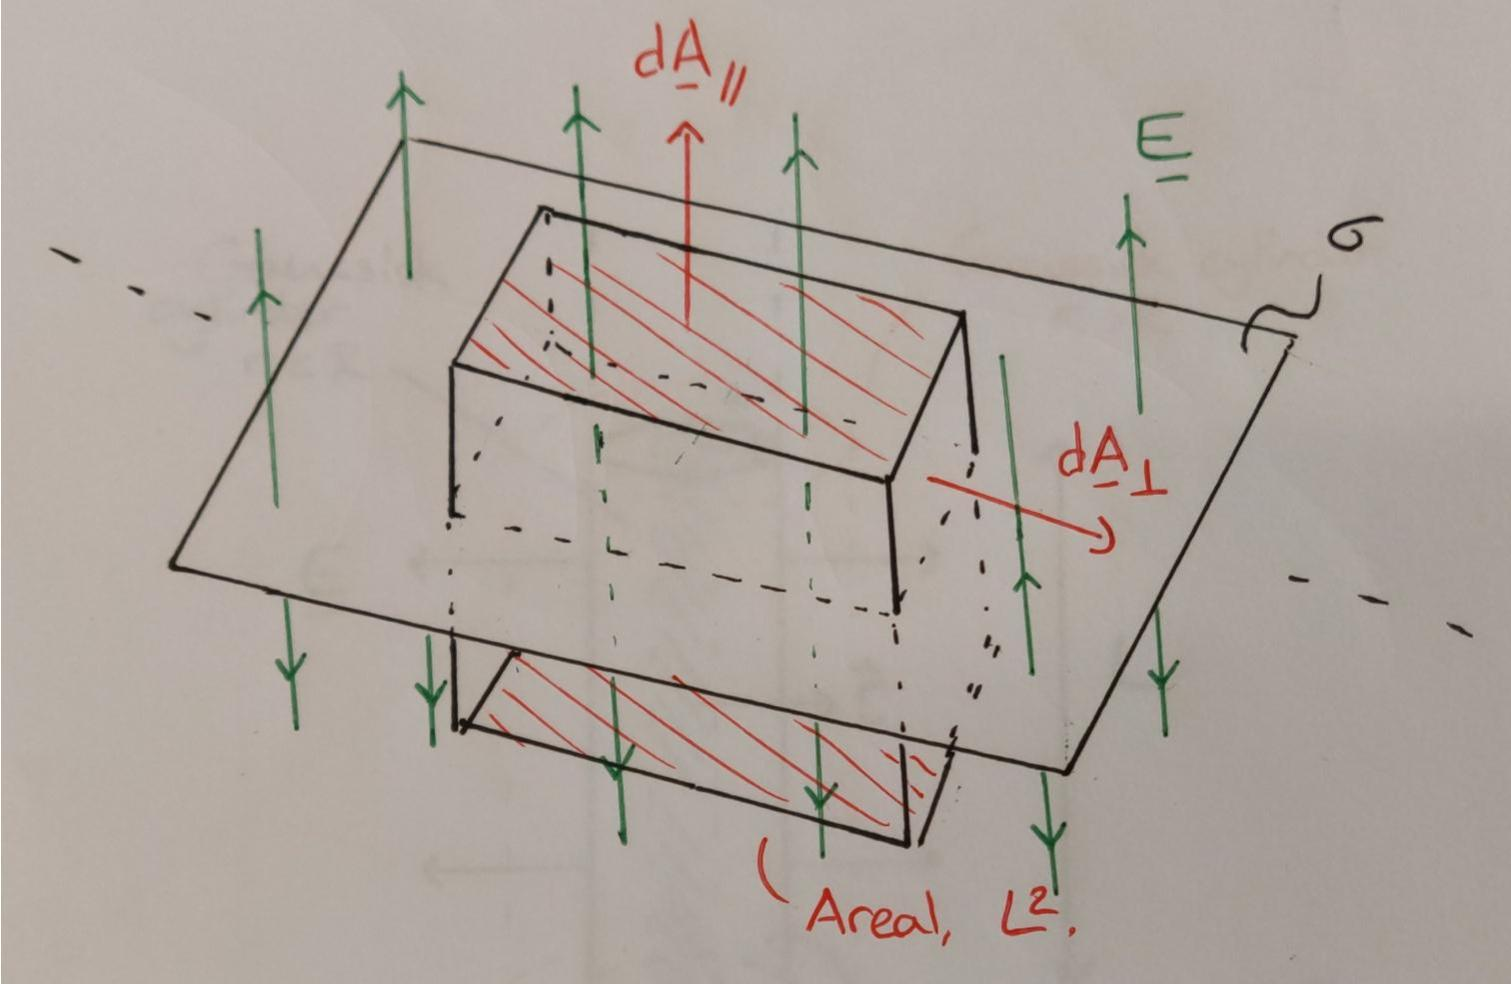
\includegraphics[width=0.8\textwidth]{facit/figurer/elektro/elektro_opg6,1.jpg}
    \end{figure}
    \opg Inde i kassen er der en kvadratisk sektion af det ladede plan, med sidelængde $L$. Arealet af planet inde i kassen er derfor $L^2$. Den samlede ladning må være
    \[ Q_\text{inde}=\sigma\cdot\text{Areal}=\sigma L^2. \]
    \opg Per symmetri kan de elektriske feltlinjer ikke pege langs planet, da feltlinjerne ville røre hinanden. Så derfor må de udelukkende pege væk fra planet.
    \opg Fire af kassens sider peger vinkelret på planet. Arealvektoren $\dd \va {A}_\perp$ peger derfor vinkelret med hensyn til de elektriske feltlinjer, så
    \[ \va E\cdot \dd\va {A}_\perp=0. \]
    Toppen og bunden af kassen er overflader der er parallelle med det ladede plan, så $\va E$ må også pege parallelt til arealvektoren, $\dd \va {A}_\parallel$.
    \[ \va E\cdot \dd\va {A}_\parallel = E\dd A_\parallel \]
    Arealet af toppen og bunden af kassen er til sammen $2L^2$, så
    \[ \oint_S \va E\dd \va {A}=2L^2E. \]
    \opg Ved brug af Gauss' lov får man
    \[ \oint_S\va E\dd \va {A}=\frac{Q_\text{inde}}{\varepsilon_0}. \]
    Bruger vi resultaterne fra forrige opgaver giver det ligningen
    \[ 2L^2E=\frac{\sigma L^2}{\varepsilon_0}. \]
    Løses for det elektriske felt, giver det
    \[ E=\frac{\sigma}{2\varepsilon_0}. \]
    Bemærk, at feltstyrken er det samme lige meget, hvor langt væk fra planet man er. Dette er kun sagen, fordi planet udspænder sig uendelig langt.\\
    Der er dog endnu et trin, hvis vi skal skrive feltstyrken som en vektor. Lad os antage, at det uendelige plan ligger i $xy$-planet (med andre ord er $z=0$). Hvis vi ser på positiv $z$, kan vi se at vektoren skal pege opad, mens hvis vi ser på negativ $z$, skal vektoren pege nedad. Derudover ligger $\va E$ altid langs $z$-enhedsvektoren, så
    \[ \va E=\begin{cases*}
    \dfrac{\sigma}{2\varepsilon_0}\vu z & for $z>0$\\
    -\dfrac{\sigma}{2\varepsilon_0}\vu z & for $z<0$
    \end{cases*}.\]
    \opg Som vi så ovenfor, er E-feltets styrke det samme overalt i rummet.
\end{opgave}

\begin{opgave}{Ladet kugle I}
    \opg Radius af den ladede kugle er $R$, da kuglen har ladningsfordelingen $\rho(r) = 0$ for $r > R$.
    \opg 
    \begin{figure}[H]
        \centering
        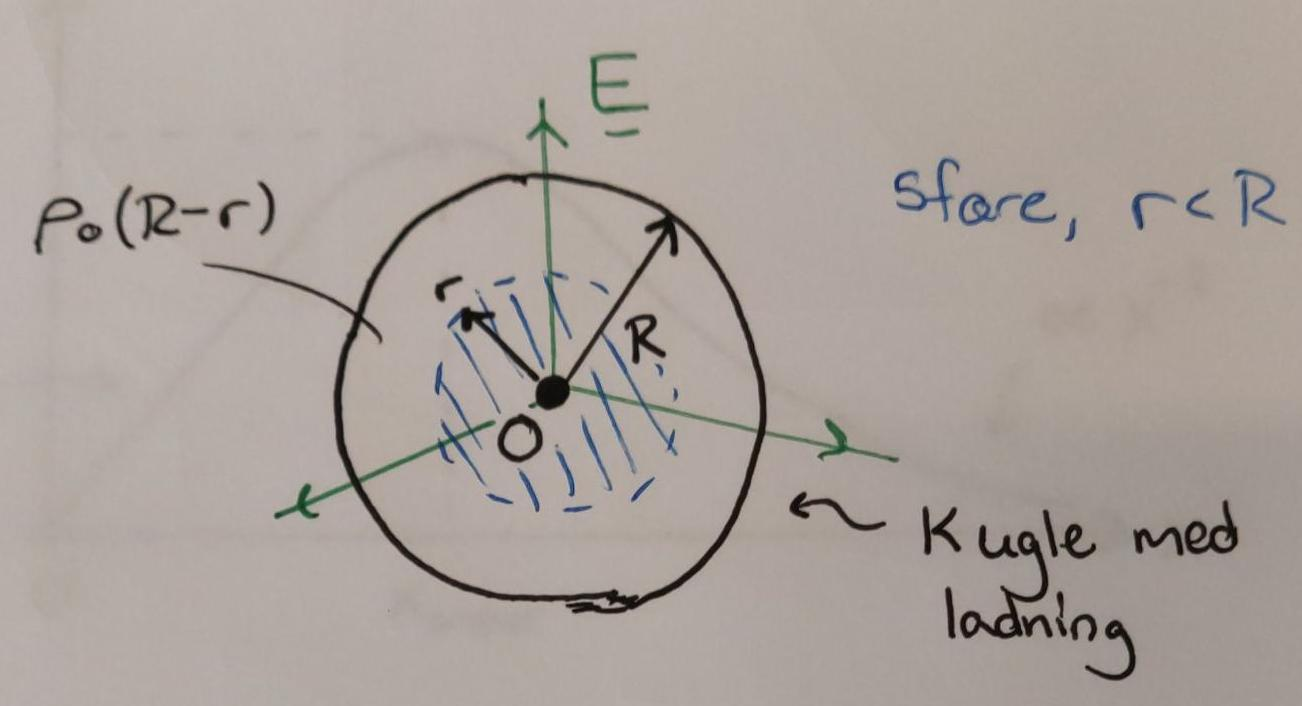
\includegraphics[width=0.49\textwidth]{facit/figurer/elektro/elektro_opg7,2(1).jpg}
        %
        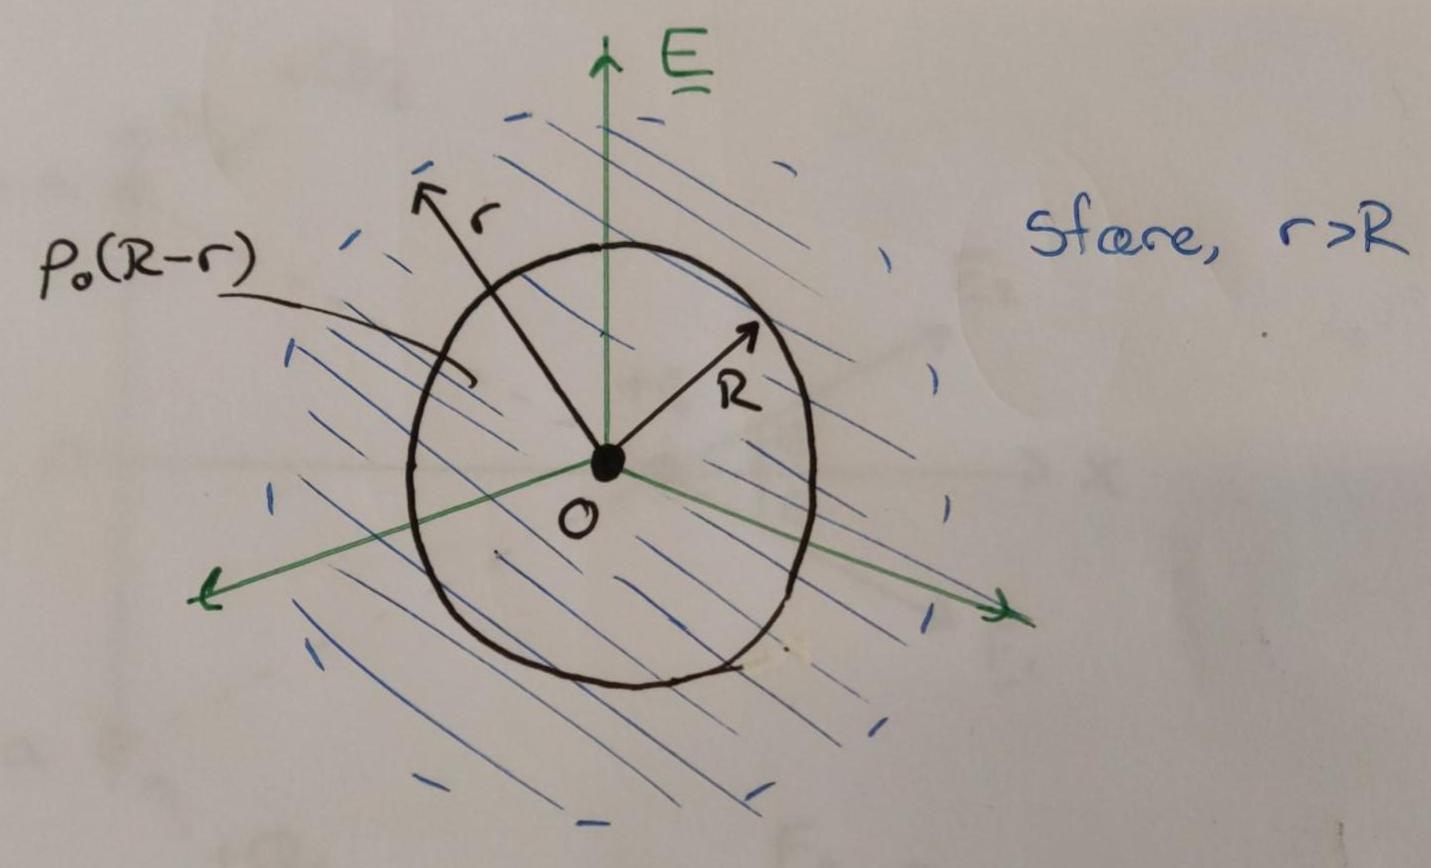
\includegraphics[width=0.49\textwidth]{facit/figurer/elektro/elektro_opg7,2(2).jpg}
    \end{figure}
    \opg Vi beregner integralet
    \begin{align*}
        Q_\text{inde}&=\int_V\rho\dd V\\
        &=\int_0^r\rho(r)4\pi r^2\dd r\\
        &=\int_0^r 4\pi\rho_0(R_0-r)r^2\dd r\\
        &=4\pi\rho_0\left(\frac{1}{3}R_0r^3-\frac{1}{4}r^4\right)
    \end{align*}
    for $r<R$.
    \opg Per symmetri skal $\va E$ pege væk fra origo.\footnote{Som en analogi, forestil dig hvordan man kan kæmme et pindsvin. Det bliver ikke muligt uden at nogle af piggene peger i en mærkelig retning. Matematisk kaldes dette også for `Hairy Ball Theorem'.}
    \opg Fordi $\va E$ peger vinkelret på overfladen, må den være parallel med arealvektoren. Så
    \[ \va E\cdot \dd\va A=E\dd A. \]
    Overfladearealet af en kugle med radius $r$ er $4\pi r^2$, så
    \[ \va E\cdot \dd\va A=4\pi Er^2. \]
    \opg Gauss' lov er
    \[ \oint \va E\cdot \dd \va A=\frac{Q_\text{inde}}{\varepsilon_0}. \]
    Bruger vi resultaterne fra forrige opgaver får vi
    \[ 4\pi r^2 E=\frac{4\pi\rho_0}{\varepsilon_0}\left(\frac{1}{3}Rr^3-\frac{1}{4}r^4\right) \]
    \[ \Rightarrow E=\frac{\rho_0 r}{\varepsilon_0}\left(\frac{1}{3}R-\frac{1}{4}r\right) \]
    for $r<R$.
    \[ \Rightarrow \va E=\frac{\rho_0 r}{\varepsilon_0}\left(\frac{1}{3}R-\frac{1}{4}r\right)\vu r \]
    \opg Det eneste vi skal beregne igen er ladningen inde i kuglen med radius $r>R$, da ladningsdensiteten er nul udenfor kuglen med radius $R$. Overfladeintegralet giver stadig
    \[ \oint \va E\cdot \dd\va A=4\pi r^2E, \]
    men når vi beregner $Q_\text{inde}/\varepsilon_0$, som er højre side af Gauss' lov, giver det
    \begin{align*}
        \frac{Q_\text{inde}}{\varepsilon_0}&=\frac{1}{\varepsilon_0}\int_0^R 4\pi\rho_0(R-r)r^2\dd r\\
        &=\frac{4\pi\rho_0}{\varepsilon_0}\underbrace{\left(\frac{1}{3}-\frac{1}{4}\right)}_{\text{$1/12$}}R^4\\
        &=\frac{\pi\rho_0}{3\varepsilon_0}R^4
    \end{align*}
    Gauss' lov giver
    \[ 4\pi r^2E=\frac{\pi\rho_0}{3\varepsilon_0}R^4. \]
    Løser vi for $E$, kan vi herefter skrive $\va E=E\vu r$.
    \[ \va E=\frac{1}{4\pi\varepsilon_0}\left(\frac{\pi}{3}\rho_0R^4\right)\frac{1}{r^2}\vu r \]
    Her ser vi at den effektive ladning er
    \[ \widetilde{Q}=\frac{\pi}{3}\rho_0R^4. \]
    \opg Dette svarer til det elektriske felt fra en punktladning $\widetilde{Q}$ placeret i origo.
\end{opgave}

\begin{opgave}{Ladet kugle II}
    \opg Der er ingen ladningsdensitet uden for kuglen. Vi har altså at gøre med en isoleret kugle af ladning.
    \opg Overfladeintegralet på kuglen med radius $r>R$ giver
    \[ \oint\va E\cdot \dd\va A=4\pi r^2E. \]
    Fordi den kugleskal vi ser på er større end selve kugleladningen, må ladningen inden i systemet svare til hele kuglens ladning. Fordi ladningsdensiteten er konstant, ved vi at den samlede ladning er $Q=\rho\cdot\text{Volumen}$, så
    \[ \frac{Q_\text{inde}}{\varepsilon_0}=\frac{4}{3}\pi R^3\rho_0\frac{1}{\varepsilon_0}. \]
    Sætter vi de to lig hinanden giver det
    \[ \va E=\frac{1}{4\pi\varepsilon_0}\underbrace{\left(\frac{4}{3}\pi R^3\rho_0\right)}_{\text{Effektiv ladning, $\tilde{Q}$}}\frac{1}{r^2}\vu r. \]
    \opg Her er ladningen inde i kugleskallen som vi integrerer over, ikke alt ladningen i kuglen. Igen kan vi gange ladningsdensitet med volumen, således at 
    \[ \frac{Q_\text{inde}}{\varepsilon_0}=\frac{4}{3}\pi r^3\rho_0\frac{1}{\varepsilon_0}. \]
    Sætter vi nu
    \[ 4\pi r^2E=\frac{Q_\text{inde}}{\varepsilon_0} \]
    og løser for $E$, giver det til sidst vektoren for den elektriske feltstyrke
    \[ \va E=\frac{\rho_0 r}{3\varepsilon_0}\vu r. \]
\end{opgave}

\begin{opgave}{Ladet cylinder}
    \opg Ligesom for den uendelige lange ladet linje, gælder der per symmetri at $\va E$ peger væk fra centrum af cylinderen.
    \begin{figure}[H]
        \centering
        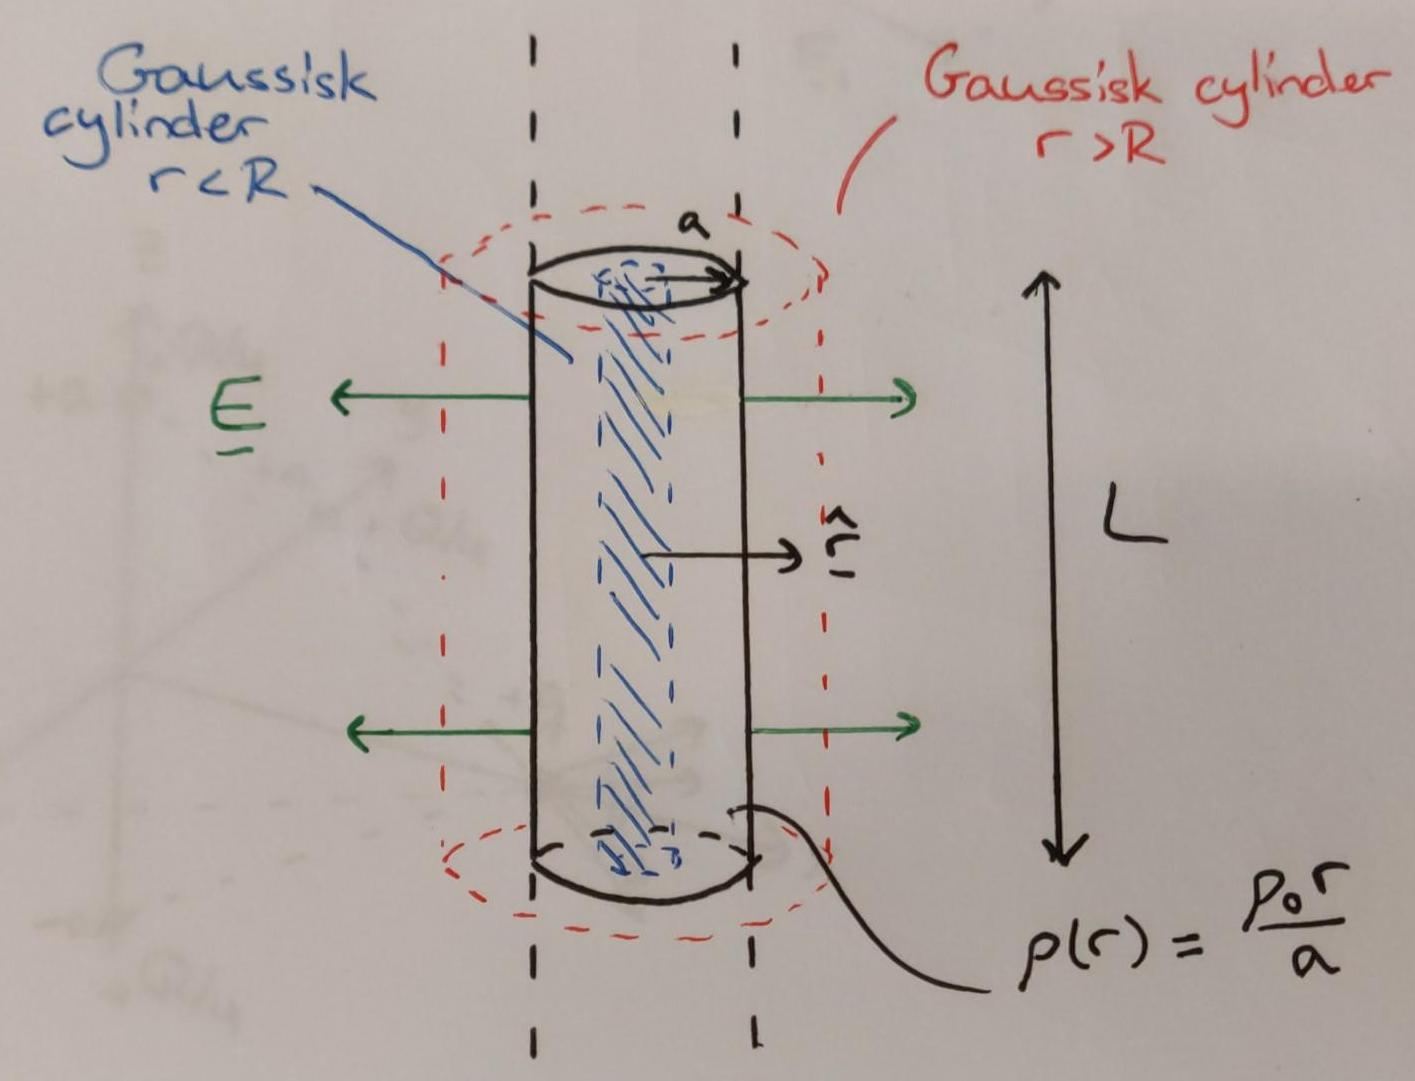
\includegraphics[width=0.8\textwidth]{facit/figurer/elektro/elektro_opg9,1.jpg}
    \end{figure}
    Betragt en $L$ lang sektion af cylinderen. Overfladeintegralet på cylinderen er
    \[ \oint \va E\cdot \dd\va A=2\pi rLE \]
    som svarer til arealet af den krumme overflade, ganget med feltstyrken, da arealvektoren på enderne af cylinderen står vinkelret på feltlinjerne, så prikproduktet er nul.\\[12pt]
    \underline{$r<a$:} Højre side af Gauss' lov giver
    \begin{align*}
        \frac{Q_\text{inde}}{\varepsilon_0}&=\frac{1}{\varepsilon_0}L\int\rho(r)\dd A\\
        &=\frac{L}{\varepsilon_0}\int_0^r\frac{\rho_0r}{a}2\pi r\dd r\\
        &=\frac{L\rho_0}{\varepsilon_0a}\frac{2\pi}{3}r^3.
    \end{align*}
    Sætter vi de to udtryk lig hinanden får man
    \[ \va E=\frac{\rho_0}{3\varepsilon_0a}r^2\vu r \]
    for $r<a$.\\[12pt]
    \underline{$r>a$:} Udenfor en radius på $a$ er ladningsdensiteten nul, så ladningen inde i den gaussiske cylinder er
    \begin{align*}
        \frac{Q_\text{inde}}{\varepsilon_0}&=\frac{L}{\varepsilon_0}\int_0^a\frac{\rho_0r}{a}2\pi r\dd r\\
        &=\frac{L\rho_0}{\varepsilon_0}\frac{2\pi}{3}a^2.
    \end{align*}
    Sættes dette lig med $2\pi rLE$ og løser man for $E$, giver det
    \[ \va E=\frac{\rho_0 a^2}{3\varepsilon_0 r}\vu r \]
    for $r>a$.
\end{opgave}

\begin{opgave}{Cylindrisk ladningsfordeling}
    \opg
    \begin{figure}[H]
        \centering
        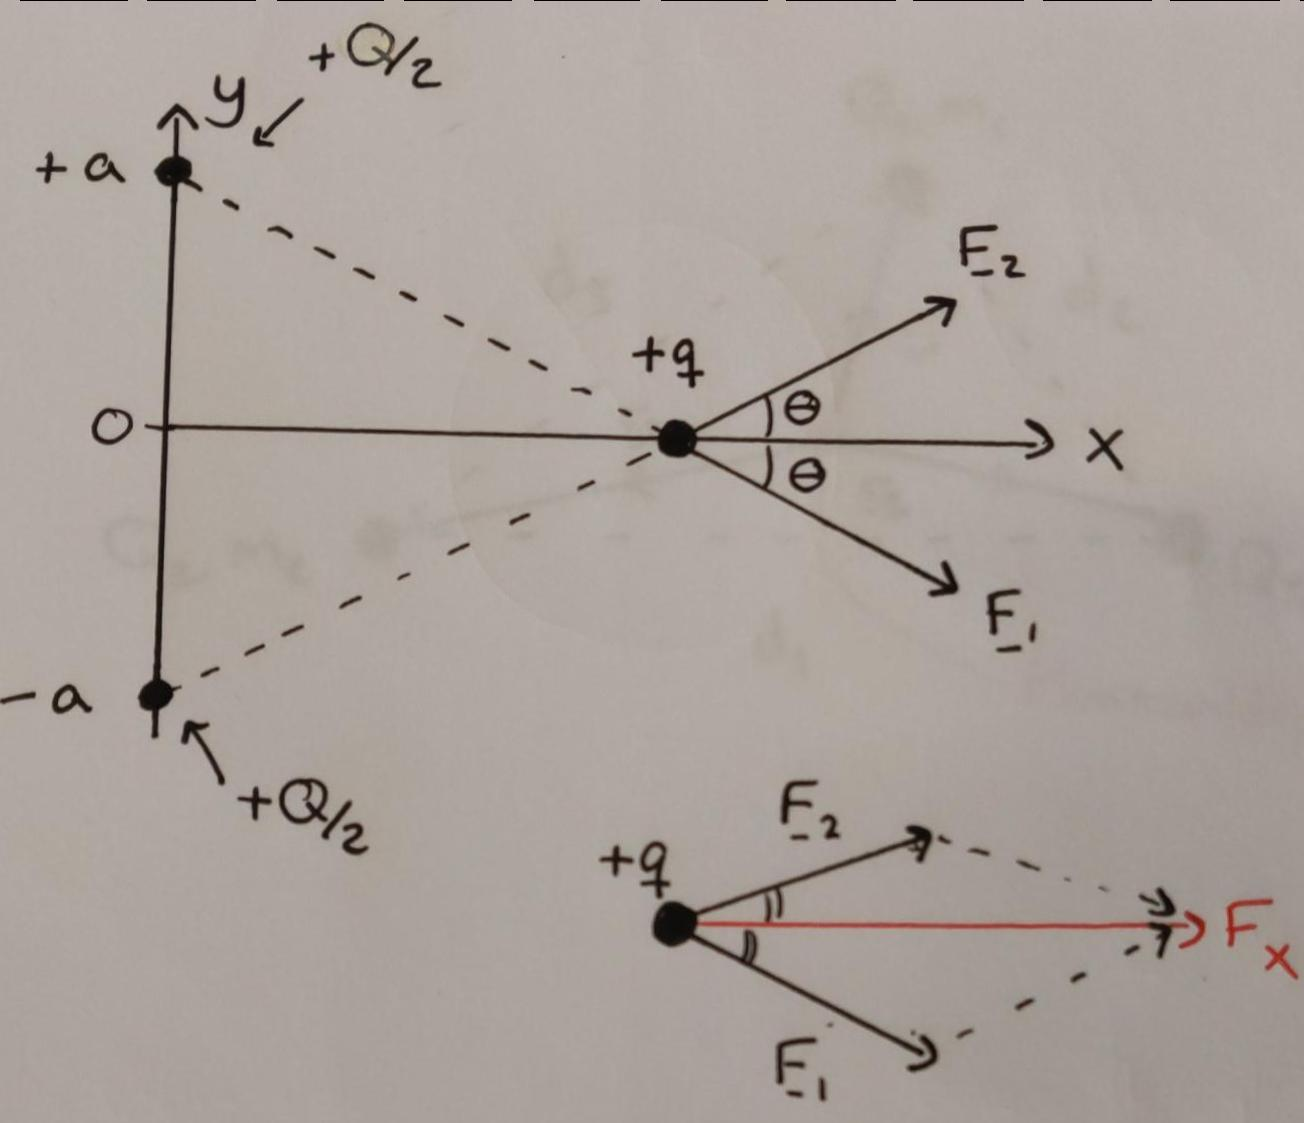
\includegraphics[width=0.8\textwidth]{facit/figurer/elektro/elektro_opg10,1.jpg}
    \end{figure}
    \opg For $x=0$ vil kraften være $F=0$ pga. symmetri.\\
    Ved $x\gg a$ vil $+q$ kun se to ladninger $+Q/2$ placeret meget tæt på hinanden, så essentielt er det en ladning $+Q$ placeret ved $x=0$. Vi forventer derfor at
    \[ F\approx\frac{1}{4\pi\varepsilon_0}\frac{Qq}{x^2}. \]
    \opg Vi ser at per symmetri vil $F_y=F_z=0$ (altså $y$ og $z$ komponenten af $\va F$). Kun $x$ komponenten $F_x$ vil ikke være nul. Ved brug af superpositionsprincippet giver denne
    \begin{align*}
        F_x&=\frac{1}{4\pi\varepsilon_0}\frac{Qq}{2}\underbrace{\left[\frac{1}{x^2+a^2}+\frac{1}{x^2+a^2}\right]}_{\text{$1/r_1^2+1/r_2^2$}}\underbrace{\frac{x}{\sqrt{x^2+a^2}}}_{\text{$\cos(\theta)$}}\\
        &=\frac{Qq}{4\pi\varepsilon_0}\frac{x}{(x^2+a^2)^{3/2}}
    \end{align*}
    \opg Vi vil gerne have, at $F(0)=0$ og
    \[ F(x\gg a)\approx\frac{1}{4\pi\varepsilon_0}\frac{Qq}{x^2}. \]
    Når $x$ er meget lille, vil $x^2\ll a^2$, så det kan vi ignorere i nævneren:
    \begin{align*}
        F_x&\approx \frac{Qq}{4\pi\varepsilon_0}\frac{x}{(a^2)^{3/2}}\\
        &=\frac{Qq}{4\pi\varepsilon_0}\frac{x}{a^3}
    \end{align*}
    Her ses at $F_x\to 0$ når $x\to 0$, som er det vi ønsker.\\
    Når $x$ er meget stor, vil $x^2\gg a^2$, så vi ignorerer i stedet $a^2$ i nævneren:
    \begin{align*}
        F_x&\approx\frac{Qq}{4\pi\varepsilon_0}\frac{x}{(x^2)^{3/2}}\\
        &=\frac{Qq}{4\pi\varepsilon_0}\frac{1}{x^2}
    \end{align*}
    Dette er Coulombs lov, som vi søgte.
    \begin{figure}[H]
        \centering
        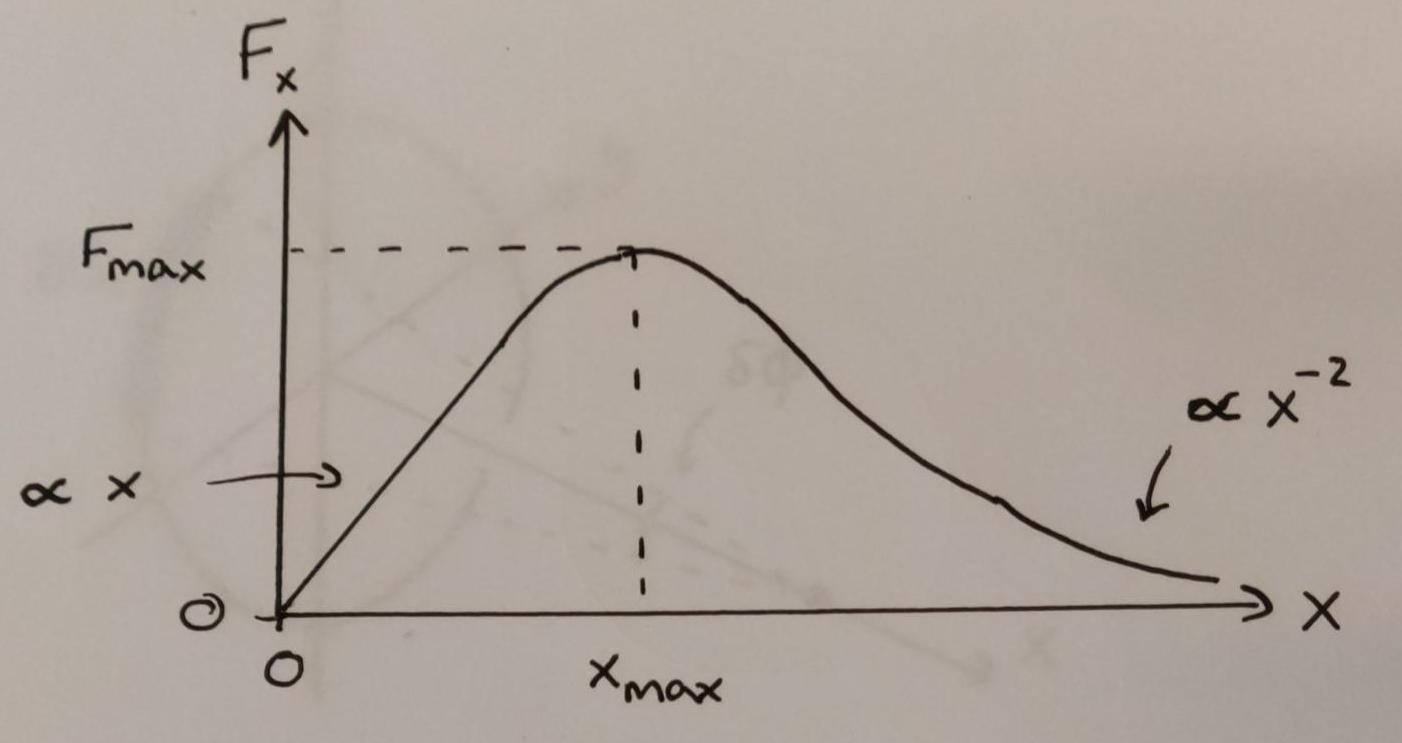
\includegraphics[width=0.8\textwidth]{facit/figurer/elektro/elektro_opg10,4.jpg}
    \end{figure}
    For at finde maksimum, differentierer vi $F_x$ med hensyn til $x$ og sætter det lig nul.
    \[ \frac{\dd F_x}{\dd x}=0=\frac{Qq}{4\pi\varepsilon_0}\left[\frac{1}{(x^2+a^2)^{3/2}}-\frac{3}{2}\frac{2x^2}{(x^2+a^2)^{5/2}}\right] \]
    Ved lidt algebraisk gymnastik får man udtrykket
    \[ 3x^2=x^2+a^2. \]
    Dette er en andengradsligning med løsning
    \[ x=\pm \frac{a}{\sqrt{2}}. \]
    \opg Igen er $F_y=F_z=0$ per symmetri. Alle $+Q/4$ ladninger har samme afstand til ladningen $+q$ og $F_x$ komponenten har samme vinkel om $x$-aksen.
    \begin{figure}[H]
        \centering
        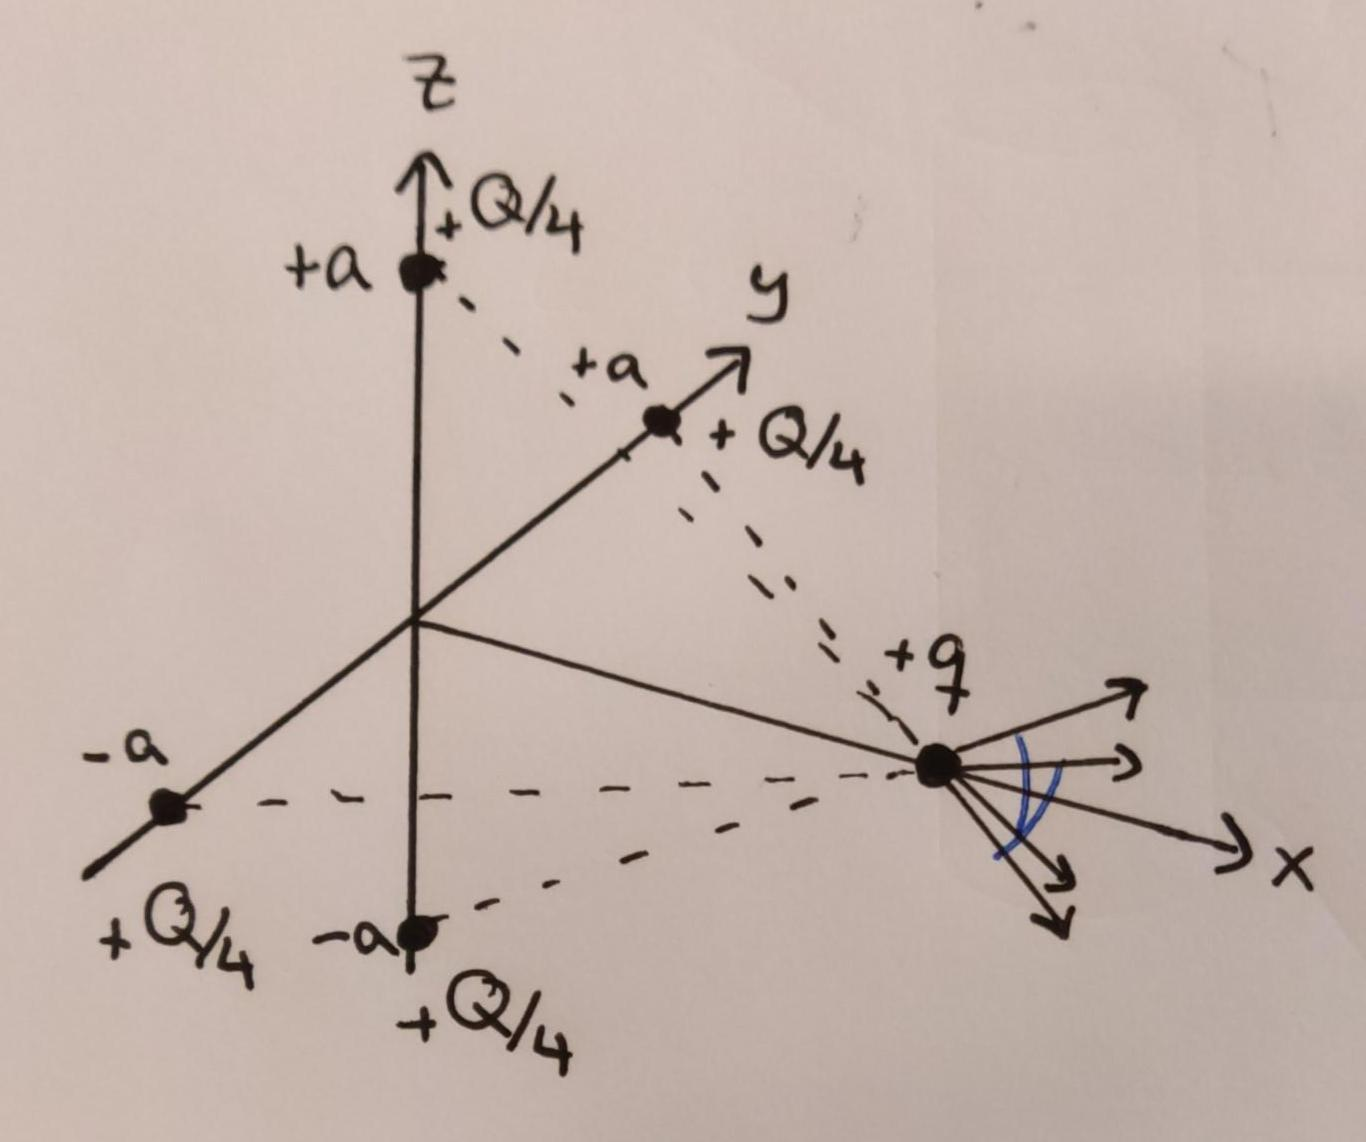
\includegraphics[width=0.8\textwidth]{facit/figurer/elektro/elektro_opg10,5.jpg}
    \end{figure}
    Ved brug af superposition får man
    \begin{align*}
        F_x&=\frac{\frac{1}{4}Qq}{4\pi\varepsilon_0}\underbrace{\left[\frac{4}{x^2+a^2}\right]}_{\text{Fire interaktioner}}\frac{x}{\sqrt{x^2+a^2}}\\
        &=\frac{Qq}{4\pi\varepsilon_0}\frac{x}{(x^2+a^2)^{3/2}}
    \end{align*}
    som er det samme udtryk som før.
    \opg Hvis vi følger ovenstående logik, får vi faktisk igen det samme resultat.
    \opg Vi gætter på at vi igen får det samme udtryk, men vi kan også prøve at vise det:
    \begin{figure}[H]
        \centering
        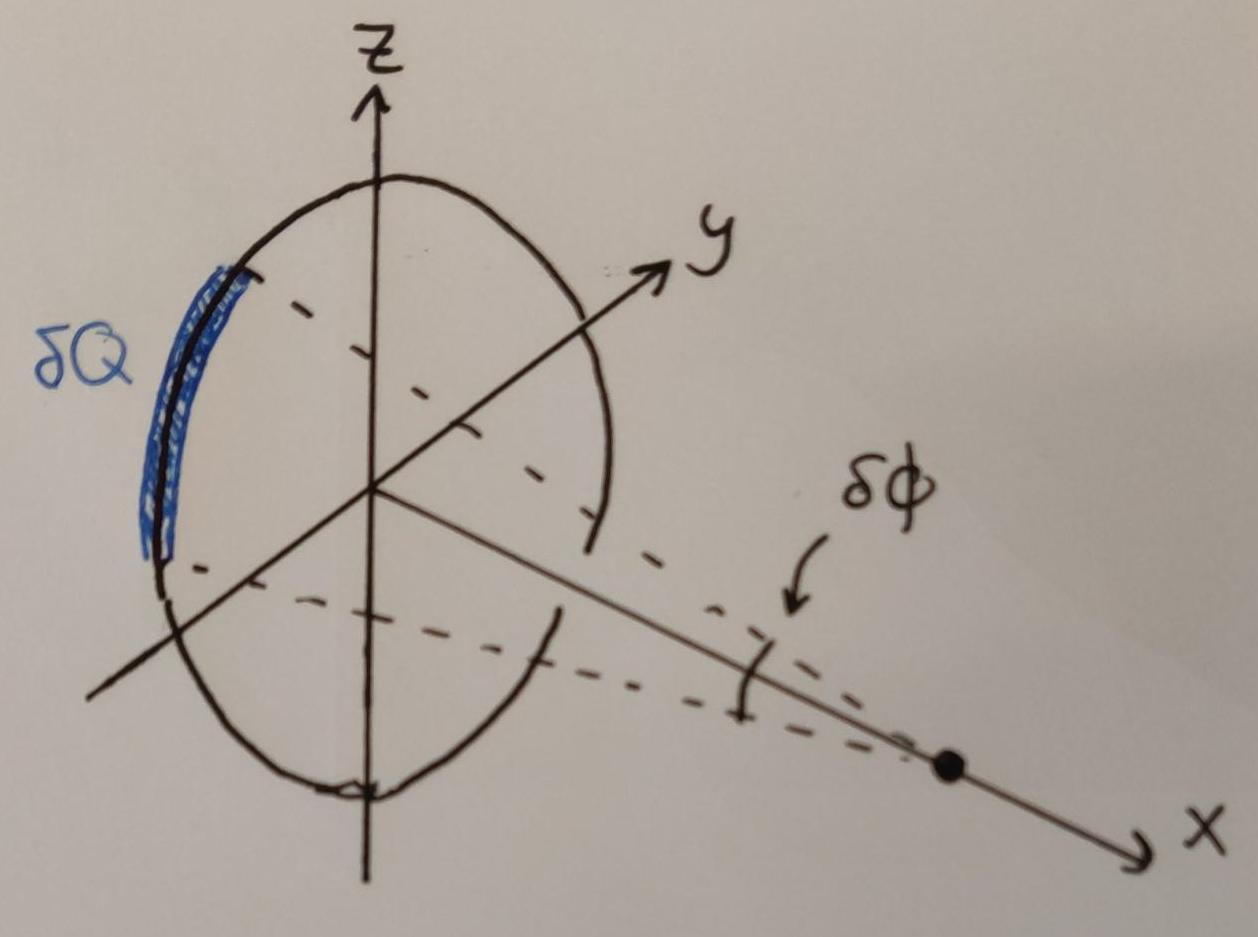
\includegraphics[width=0.8\textwidth]{facit/figurer/elektro/elektro_opg10,7.jpg}
    \end{figure}
    Betragt et infinitesimalt stykke ladning $\delta Q$ langs en cirkel, som tilsammen spænder en vinkel $\delta\phi$. Hvis cirklens totale ladning er $Q$, gælder
    \[ \delta Q=Q\cdot \frac{\delta \phi}{2\pi}. \]
    Kraften forårsaget af det lille stykke ladning må, som vi tidligere har udledt, svare til
    \[ \delta F_x=\frac{\delta Q q}{4\pi\varepsilon_0}\frac{x}{(x^2+a^2)^{3/2}}. \]
    Hvis vi integrerer over hele cirklen, altså en vinkel fra 0 til $2\pi$, må man få hele kraften
    \[ F_x=\int_0^{2\pi}\delta F_x=\frac{Qq}{4\pi\varepsilon_0}\frac{x}{(x^2+a^2)^{3/2}}. \]
    Dette er resultatet som vi gættede.
    \opg Vi kan betragte disken som en masse individuelle ringe af ladning, hver med tykkelse $\delta r$. Ladningen af hver ring er
    \[ Q_\text{ring}=Q\cdot\frac{2\pi r\delta r}{\pi a^2}=\frac{2Qr}{a^2}\delta r, \]
    hvor $Q$ er diskens totale ladning. Så hver ring (med radius $r$) skubber med en kraft
    \begin{align*}
        \delta F_x&=\frac{Q_\text{ring}q}{4\pi\varepsilon_0}\frac{x}{(x^2+r^2)^{3/2}}\\
        &=\frac{Qqrx}{2\pi a^2\varepsilon_0}\frac{1}{(x^2+r^2)^{3/2}}\delta r.
    \end{align*}
    Den samlede kraft pga. alle ringe må derfor være
    \begin{align*}
        F_x&=\frac{Qqx}{2\pi a^2\varepsilon_0}\int_0^a\frac{r}{(x^2+r^2)^{3/2}}\dd r\\
        &=\frac{Qqx}{2\pi a^2\varepsilon_0}\left[-\frac{1}{\sqrt{x^2+r^2}}\right]_0^a\\
        &=\frac{Qq}{2\pi a^2\varepsilon_0}\left(1-\frac{x}{\sqrt{x^2+a^2}}\right).
    \end{align*}
\end{opgave}

\begin{opgave}{Ladede partikler i en trekant}
    \begin{figure}[H]
        \centering
        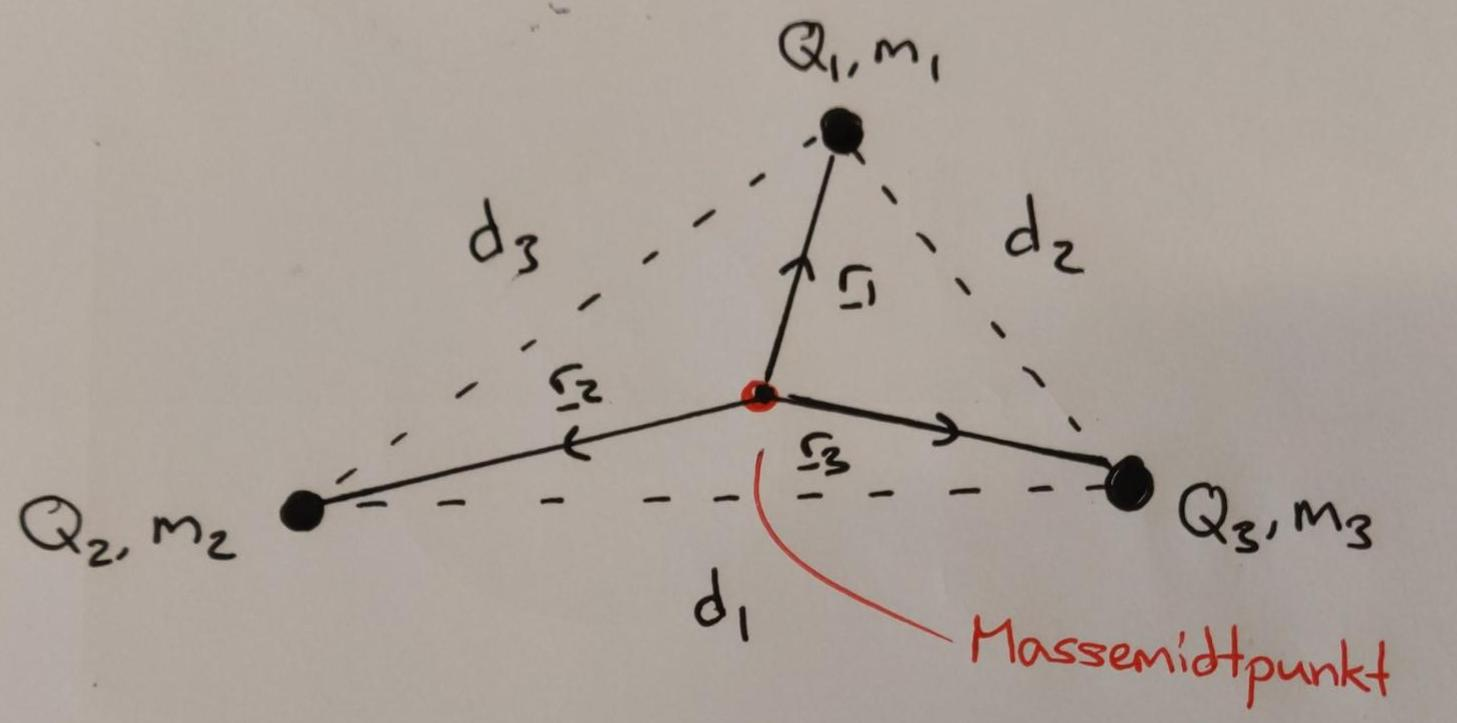
\includegraphics[width=0.8\textwidth]{facit/figurer/elektro/elektro_opg11.jpg}
    \end{figure}
    Før vi starter med at løse opgaven, giver det god mening af vælge et reference system, når vi ser på vores vektorer. Da alle ladninger flytter sig relativt til hinanden, er det ikke særligt smart at vælge én partikel som origo. Til gengæld viser det sig at være smart, hvis vi vælger massemidtpunktet til at være centrum. Vi noterer at:
    \begin{enumerate}
        \item Der er ingen eksterne krafter på partiklerne, så massemidtpunktet flytter sig aldrig!
        \item Med massemidtpunktet som reference, hvis en partikel bevæger sig i en lige linje, så vil accelerationsvektoren være parallel med positionsvektoren, $\va a\parallel \va r$.
        \item Hvis $\frac{\abs{\va r_i}}{\abs{\va r_j}}$ er konstant for alle $i,j=1,2,3$, så må trekanten være ens hele tiden.\footnote{Med andre ord, hvis forholdene mellem sider på trekanten er konstant, må trekanten til enhver tid være kongruente.}
    \end{enumerate}
    For nemhedens skyld vil vi bruge notationen for Coulombs konstant
    \[ k_c=\frac{1}{4\pi\varepsilon_0}. \]
    Ved brug af superpositionsprincippet og Newtons lov, kan vi skrive kraften på partikel 1 som
    \[ \va F_1=m_1\va a_1=k_c\frac{Q_1Q_2}{d_3^3}(\va r_1-\va r_2)+k_c\frac{Q_1Q_3}{d_2^3}(\va r_1-\va r_3). \]
    Massemidtpunktet kan vi definere på flere forskellige måder:
    \[ \sum_{i=1}^3 m_i\va a_i=\sum_{i=1}^3 m_i\va v_i=\sum_{i=1}^3 m_i \va r_i=0 \]
    Hvis vi substituerer
    \[ \va r_3=-\frac{1}{m_3}\left(m_1\va r_1+ m_2\va r_2\right) \]
    ind i kraftudtrykket får man
    \begin{align*} 
        m_1\va a_1&=k_cQ_1\left(\frac{Q_2}{d_3^3}(\va r_1-\va r_2)+\frac{Q_3}{d_2^3}\left(\va r_1+\frac{m_1}{m_3}\va r_1+\frac{m_2}{m_3}\va r_2\right)\right)\\
        &=k_cQ_1\left[\frac{Q_2}{d_3^3}+\frac{Q_3}{d_2^3}\left(\frac{m_1}{m_3}+1\right)\right]\va r_1 +k_cQ_1\left[\frac{Q_3}{d_2^3}\frac{m_2}{m_3}-\frac{Q_2}{d_3^3}\right]\va r_2.
    \end{align*}
    Hvis partiklerne bevæger sig i en lige linje må det betyde, at $\va a_1$ skal have samme retning som $\va r_1$. I så fald skal komponenten foran $\va r_2$ give 0.
    \[ \frac{Q_3}{d_2^3}\frac{m_2}{m_3}=\frac{Q_2}{d_3^3} \]
    Ved at bytte rundt på variabler i ligningen, og vise samme slags ligninger for de to andre partikler, kan man vise at
    \[ \frac{Q_1d_1^3}{m_1}=\frac{Q_2d_2^3}{m_2}=\frac{Q_3d_3^3}{m_3}. \]
    Med andre ord skal
    \[ \frac{d_1}{d_2}=\sqrt[3]{\frac{Q_2m_1}{Q_1m_2}}=\text{konstant} \]
    \[ \frac{d_2}{d_3}=\sqrt[3]{\frac{Q_3m_2}{Q_2m_3}}=\text{konstant} \]
    \[ \frac{d_3}{d_1}=\sqrt[3]{\frac{Q_1m_3}{Q_3m_1}}=\text{konstant} \]
    Altså har siderne i trekanten konstante forhold. Så trekanten til enhver tid efter vi har sluppet partiklerne må være kongruent til den originale trekant.
\end{opgave}


\subsection*{Magnetisme}

\begin{opgave}{Magnetisk felt}
    \opg Indsættes tallene i formlen fås:
    \begin{enumerate}
        \item $\va B(\va r) = \dfrac{\mu_0}{4\pi}\dfrac{qv\xhat \times r\xhat}{r^3} = \SI{0,00}{\tesla}$.
        \item $\va B(\va r) = \dfrac{\mu_0}{4\pi}\dfrac{qv\xhat \times r\yhat}{r^3} = \SI{1,00e-7}{\tesla}\cdot \zhat$.
        \item $\va B(\va r) = \dfrac{\mu_0}{4\pi}\dfrac{qv\xhat \times r\zhat}{r^3} = -\SI{1,00e-7}{\tesla}\cdot \yhat$.
        \item $\va B(\va r) = \dfrac{\mu_0}{4\pi}\dfrac{qv\xhat \times r\yhat}{r^3} = -\SI{1,00e-7}{\tesla}\cdot \zhat$.
        \item $\va B(\va r) = \dfrac{\mu_0}{4\pi}\dfrac{qv\xhat \times r\yhat}{r^3} = \SI{2,00e-7}{\tesla}\cdot \zhat$.
        \item $\va B(\va r) = \dfrac{\mu_0}{4\pi}\dfrac{qv\xhat \times r\yhat}{r^3} = \SI{2,00e-7}{\tesla}\cdot \zhat$.
        \item $\va B(\va r) = \dfrac{\mu_0}{4\pi}\dfrac{qv\xhat \times r\yhat}{r^3} = \SI{2,50e-8}{\tesla}\cdot \zhat$.
    \end{enumerate}
    \opg Når ladningen skifter fortegn skifter feltet retning. Når ladningen eller farten fordobles gør feltstyrken ligeså. Ændres bevægelsesretning, ændres feltets retning også, således at feltet stadig står vinkelret på stedvektoren og hastighedsvektoren. Fordobles afstanden bliver feltstyrken en fjerdedel af hvad det var før.
    \opg Indsættes tallene i formlen fås:
    \begin{enumerate}
        \item $\va F_{mag} = Q\va v' \times \va B(\va r) = \SI{0,00}{\newton}$.
        \item $\va F_{mag} = Q\va v' \times \va B(\va r) = -\SI{0,00}{\newton}$.
        \item $\va F_{mag} = Q\va v' \times \va B(\va r) = \SI{1,00e-7}{\newton}\cdot \xhat$.
        \item $\va F_{mag} = Q\va v' \times \va B(\va r) = \SI{0,00}{\newton}$.
        \item $\va F_{mag} = Q\va v' \times \va B(\va r) = \SI{0,00}{\newton}$.
        \item $\va F_{mag} = Q\va v' \times \va B(\va r) = \SI{0,00}{\newton}$.
        \item $\va F_{mag} = Q\va v' \times \va B(\va r) = \SI{0,00}{\newton}$.
    \end{enumerate}
    Det bemærkes at opgaven er en smule intetsigende, men ændres hastigheden til $\va{v}' = \SI{1,00}{\metre\per\second}\cdot\xhat$ fås et mere informativt resultat:
    \begin{enumerate}
        \item $\va F_{mag} = Q\va v' \times \va B(\va r) = \SI{0,00}{\newton}$.
        \item $\va F_{mag} = Q\va v' \times \va B(\va r) = -\SI{1,00e-7}{\newton}\cdot\yhat$.
        \item $\va F_{mag} = Q\va v' \times \va B(\va r) = -\SI{1,00e-7}{\newton}\cdot \zhat$.
        \item $\va F_{mag} = Q\va v' \times \va B(\va r) = \SI{1,00e-7}{\newton}\cdot \yhat$.
        \item $\va F_{mag} = Q\va v' \times \va B(\va r) = -\SI{2,00e-7}{\newton}\cdot \yhat$.
        \item $\va F_{mag} = Q\va v' \times \va B(\va r) = -\SI{2,00e-7}{\newton}\cdot \yhat$.
        \item $\va F_{mag} = Q\va v' \times \va B(\va r) = -\SI{2,50e-8}{\newton}\cdot \yhat$.
    \end{enumerate}
\end{opgave}

\begin{figure}
    \centering
    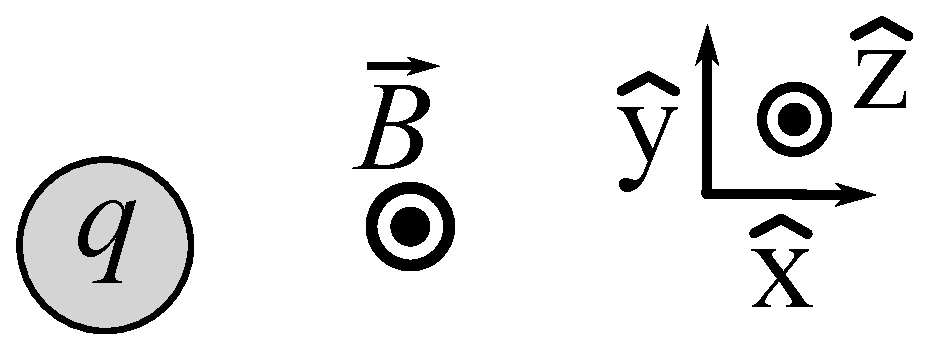
\includegraphics[width=.6\columnwidth]{facit/figurer/elektro/uniformt_felt.eps}
    \caption{Punktladning i uniformt magnetfelt.}
    \label{fig:uniformt_b-felt}
\end{figure}
%
\begin{opgave}{Uniformt magnetfelt}
    \opg Se figur \ref{fig:uniformt_b-felt}.
    \opg Feltet er uniformt, hvilket betyder at det er uafhængigt af sted. Der er derfor ingen grund til at bekymre sig om det.
    \opg Kraften, og dermed accelerationen, står altid vinkelret på feltet og hastigheden. Det samme gør sig gældende, hvis man spænder en sten fast i en snor og derefter får stenen til at dreje rundt. Stenen vil gerne fortsætte i den retning den har, men snoren trække den hele tiden ind mod ens hånd. Denne retning ændrer sig hele tiden, hvorfor bevægelsen kontinuerligt bliver afbøjet ind mod et punkt. Dette betyder at stenen kommer til at bevæge sig langs en cirkel. Det samme sker for ladningen i dette tilfælde. Den bliver hele tiden trukket mod et punkt, men pga. dens hastighed rammer den hele tiden ved siden af og ender med at være fastholdt i en cirkelbevægelse.
    \opg Ladningen ville i så fald blive accelereret med konstant acceleration i $z$-retningen, hvilket giver en parabelbevægelse -- se opgave \thechapter\ref{opg:EvsB}. Dette er det samme som tyngdekraften, hvorfor ladningen vil opføre sig som et skråt kast.
\end{opgave}

%
\begin{figure}
    \centering
    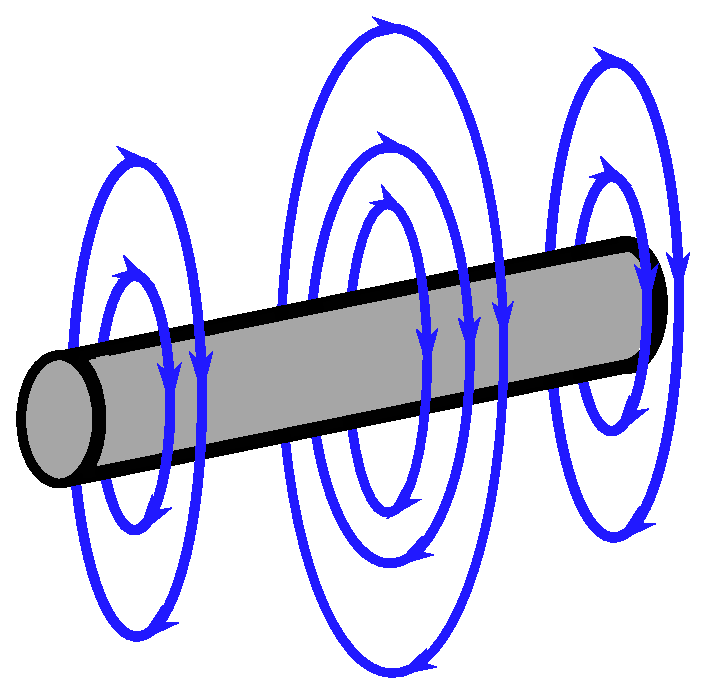
\includegraphics[width=.5\columnwidth]{facit/figurer/lige_leder.eps}
    \caption{Endelig lige leder med dens magnetiske feltlinjer i blå.}
    \label{fig:lige leder}
\end{figure}
%
\begin{opgave}{Amperes lov}
    Der er to vigtige argumenter i \ref{sec:lang_lige_leder} og alt kommer fra lederens symmetri og antagelsen om at den er uendelig lang. Forklar i det eget sprog argumenterne for at
    \opg Lederen er uendeligt lang, strømstyrken er den samme hele vejen igennem og cylindrisk symmetrisk. Det betyder at man ikke kan se forskel på forskellige steder på lederen. Feltet skal have samme symmetri, hvorfor man ikke vil kunne se forskel på feltet forskellige steder i retningen langs med lederen. Det betyder at feltet ikke kan have nogen komposant i retningen langs med lederen -- med andre ord går feltet rundt om lederen i et plan vinkelret på lederen og har form som enten ellipser eller cirkler. Da lederen er cylindrisk symmetrisk, kan man heller ikke se forskel på hvilken retning man kigger væk fra lederen. Står man i midten af en ellipse, ser den ikke ens ud i alle retninger, hvorfor den ikke har den korrekte symmetri. Den eneste mulige form feltlinjerne kan have er derfor cirkler med lederen i centrum.
    \opg Det tredimensionelle rum kan beskrives med tre koordinater. Det kan være de kartetiske $(x,y,z)$, men også de cylindriske koordinater $(r,\phi,z)$, hvor $r$ er afstanden vinkelret fra lederen, $\phi$ er den vinkel, der fortæller i hvilken retning vinkelret fra lederen man kigger, og $z$ er koordinatet langs lederen. Af ovenstående ser situationen ens ud ligegyldigt hvilket $z$-koordinat man vælger -- ergo må feltet være uafhængig at $z$. Ligeledes må de se ens ud ligegyldig hvilket $\phi$ man vælger, hvorfor feltet heller ikke må afhænge af dette koordinat. Feltet er dog ikke ens i hele rummet, da feltstyrker afhænger af hvor langt man er fra lederen, men dette er det eneste koordinat feltstørrelsen afhænger af.
    \opg Se figur \ref{fig:lige leder}.
\end{opgave}

\begin{figure}
    \centering
    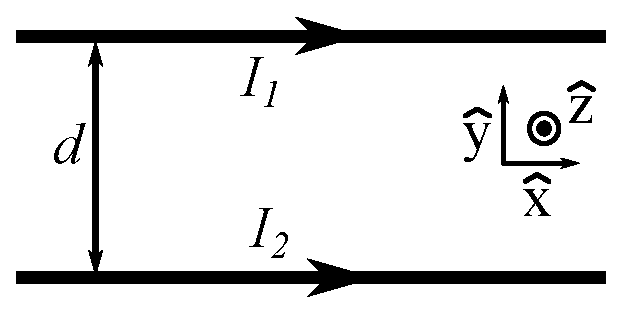
\includegraphics[width=.5\columnwidth]{facit/figurer/elektro/to_lange_lige_leder.eps}
    \caption{Skitse af situationen med de to lange lige ledere.}
    \label{fig:to_lange_lige_ledere}
\end{figure}
\begin{opgave}{To lange lige ledere}
    \opg Se figur \ref{fig:to_lange_lige_ledere}.
    \opg Se figur \ref{fig:to_lange_lige_ledere}.
    \opg Magnetfeltet fra en lang lige leder er givet ved ligning \eqref{eq:lang_lige_leder}, og af højrehåndsreglen er magnetfeltet fra den øverste leder på den nederste
    %
    \begin{align*}
        \va B = -\frac{\mu_0I_1}{2\pi d}\zhat.
    \end{align*}
    %
    \opg Da $\va I_2 = I_2\xhat$ så bevæger ladningerne sig i positiv $x$-retning. Det betyder at $\va v \times \va B \parallel \xhat \times (-\zhat) = \yhat$, hvilket er i retning af den anden leder. Ergo tiltrækkes lederne af hinanden. Dette kan også argumenteres med højrehåndsreglen for krydsproduktet.
    \opg I så fald ville der komme et ekstra fortegn i krydsproduktet, hvorved $\va v \times \va B \parallel (-\xhat) \times (-\zhat) = -\yhat$, hvorfor de frastøder hinanden. Igen fås det samme med højrehåndsreglen.
    \opg $x$-aksen placeres parallelt med den øverste leder. Det betyder at denne leder har $y$-koordinat $y_1 = 0$, mens den nederste leder har $y$-koordinat $y_2 = -d$. Da det ikke nødvendigvis er trivielt hvordan fortegnene ordner sig tages det i tre tilfælde. Først kigges på $y>0$: Her er giver begge ledere et bidrag i positiv $z$-retning, hvilket kan ses med højrehåndsreglen, hvorfor superpositionsprincippet giver at
    %
    \begin{align*}
        \va B = \frac{\mu_0}{2\pi}\left(\frac{I_1}{y} + \frac{I_2}{y+d}\right)\zhat \quad , \quad y > 0.
    \end{align*}
    %
    For $y<-d$ fås tilsvarende at
    %
    \begin{align*}
        \va B = \frac{\mu_0}{2\pi}\left(\frac{I_1}{y} + \frac{I_2}{y-d}\right)\zhat \quad , \quad y < -d.
    \end{align*}
    %
    Bemærk at feltet her peger i negativ $z$-retning da både $y$ og $y-d$ er negative tal. I tilfældet $-d<y<0$ giver de to ledere et bidrag i hver sin retning. $I_1$ giver et bidrag i negativ $z$-retning, hvilket det negative $y$-koordinat sørger for. $I_2$ giver et bidrag i positiv $z$-retning. Dette fås med feltet
    %
    \begin{align*}
        \va B = \frac{\mu_0}{2\pi}\left(\frac{I_1}{y} + \frac{I_2}{y+d}\right)\zhat \quad , \quad -d < y < 0.
    \end{align*}
    %
    Som test indsættes $y = -d/2$, hvorved det første led bliver negativt, mens det andet led bliver positivt. Yderligere går det andet led mod uendeligt i grænsen $y \rightarrow -d$, hvorfor den korrekte konstellation er opnået. Samles det fås at magnetfeltet i $xy$-planen er
    %
    \begin{align}
        \va B(y) = \begin{cases}
            \frac{\mu_0}{2\pi}\left(\frac{I_1}{y} + \frac{I_2}{y+d}\right)\zhat, \quad &y>-d \\
            \frac{\mu_0}{2\pi}\left(\frac{I_1}{y} + \frac{I_2}{y+d}\right)\zhat, \quad &y<-d
        \end{cases}
        .
    \end{align}
    %
\end{opgave}

\begin{opgave}{Forskellen på elektriske og magnetiske felter} \label{opg:EvsB}
    \opg Da feltet er homogent, har det samme størrelse og retning overalt i rummet. Lad $\vu e$ betegne en enhedsvektor i det elektriske felts retning, da kan feltet skrives som $\va E = E\vu e$. Af ligning \eqref{eq:e-felt_def} er kraften på en ladning $q$
    %
    \begin{align*}
        \va F = qE\vu e,
    \end{align*}
    %
    hvor længden af vektoren er konstant. Kaldes ladningens masse $m$ kan Newtons 2. lov, ligning \eqref{mat:eq:N2}, bruges til at bestemme accelerationen af ladningen:
    %
    \begin{align*}
        \dv[2]{\va r}{t} = \va a = \frac{qE}{m}\vu e.
    \end{align*}
    %
    Dette er en differentialligning, der kan løses ud fra tabel \ref{mat:tab:diffligninger}, hvorefter man får
    %
    \begin{align*}
        \va r(t) = \frac{1}{2}\frac{qE}{m}t^2\vu e + \va v_0 t + \va r_0,
    \end{align*}
    %
    hvor $\va v_0$ er hastigheden til tiden $t=0$, hvor feltet tændes, og $\va r_0$ er positionen til samme tid. Dette genkendes som en parabel, hvormed det ønskede er vist.
    \opg Først og fremmest bemærkes det at bevægelsen er afhængig af partiklens hastighed i stedet for at være uafhængig af sted og hastighed. Det er derfor sværere at løse differentialligningen generelt, men ikke umuligt. Elektriske felter påvirker ladninger med en kraft i samme retning som feltet. Grundet krydsproduktet i ligning \eqref{eq:magnetisk_kraft} er kraften altid vinkelret på ladningens bevægelsesretning. Dette er karakteristisk for en cirkelbevægelse omkring feltets akse. Er der tale om et homogent magnetisk felt fås derfor en spiralbevægelse omkring feltets akse, og i tilfældet hvor starthastigheden i $z$-retningen er $v_z = 0$ er ladningen i jævn cirkelbevægelsen.
    \opg I dette tilfælde er $\va v \parallel \va B$. Krydsproduktet af to parallelle vektorer er altid nul, $\va v \times \va B = \va 0$, hvorfor ladningen ikke vil blive påvirket af feltet.
\end{opgave}

\begin{opgave}{Lang lige leder med udstrækning}
    I afsnit \ref{sec:lang_lige_leder} blev det magnetiske felt fra en uendelig tynd lang lige leder bestemt. Situationen ændrer sig en smule, hvis lederen har en endelig tykkelse $R$.
    \opg Retningen på feltet ændrer sig ikke af at lederen ikke er uendelig tynd, hvorfor $\oint \va B \cdot \dd \va l$ forbliver uændret. Strømmen $I$ er nu fordelt ud over en leder, men så længe Ampereløkken er udenfor lederen, er der ikke ændret på hvor meget strøm, der er inden i lederen hvorfor $I_\mathrm{inde}$ forbliver uændret. Derved er udregningen og således resultatet helt det samme for $r>R$.
    \opg Af ovenstående sker der intet nyt udenfor lederen. Indenfor lederen er magnetfeltet stadig cirkulært, da magnetfeltet har samme cylindriske symmetri som lederen, hvorfor feltet alle steder er parallelt med integrationslinjen. Integralet bliver derfor cirklens omkreds gange feltstyrken,
    %
    \begin{align}
        \oint \va B \cdot \dd \va l = 2\pi B r.
    \end{align}
    %
    \opg Strømtætheden over cylinderens tværsnit er af ligning \eqref{eq:current_density} $J = I/\pi R^2$. Da strømmen er uniformt fordelt, så er $J$ konstant over hele tværsnittet. Derfor er
    %
    \begin{align}
        I_\mathrm{inde} = JA_\mathrm{inde}= \frac{I}{2\pi R^2} 2\pi r^2 = I \frac{r^2}{R^2}.
    \end{align}
    %
    \opg Bruges Amperes lov fås nu at for $r<R$ er
    %
    \begin{align*}
        \oint \va B \cdot \dd \va l = \mu_0I_\mathrm{inde} \implies 2\pi B r = \mu_0I \frac{r^2}{R^2} \implies B = \frac{\mu_0Ir}{2\pi R^2}.
    \end{align*}
    %
    Af spørgsmål 1 fås således at
    %
    \begin{align*}
        B = \begin{cases}
            \mu_0I/2\pi r, \qquad &r>R \\
            \mu_0Ir/2\pi R^2, \quad &r<R
        \end{cases}
        .
    \end{align*}
    %
    \begin{figure}
        \centering
        \begin{subfigure}[t]{.47\textwidth}
            \centering
            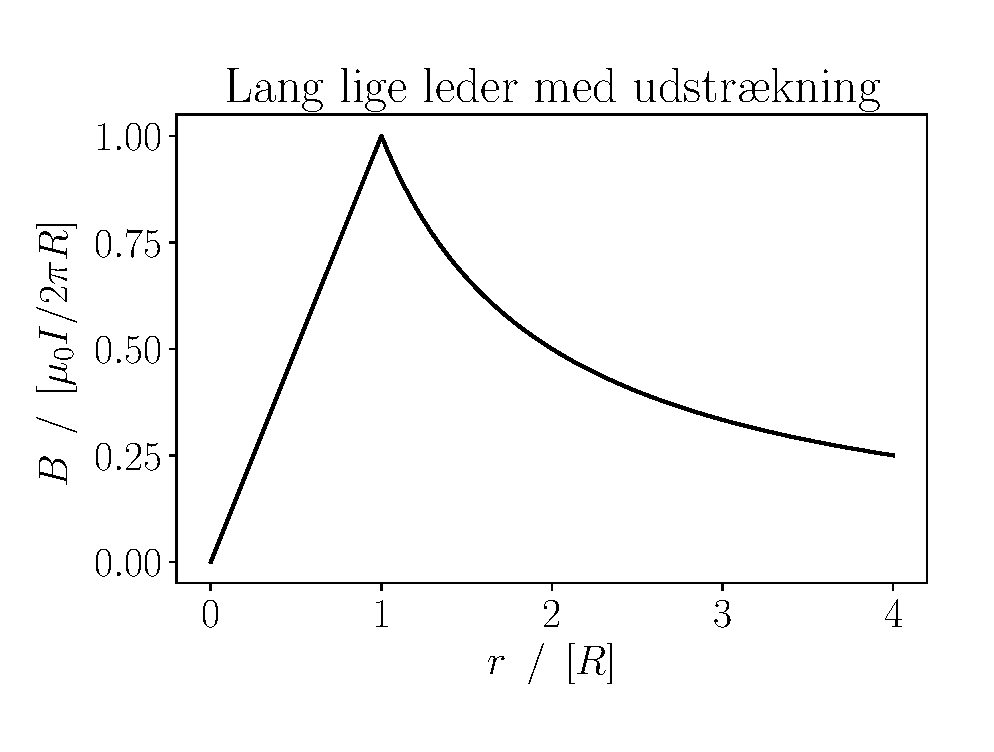
\includegraphics[width=\columnwidth]{facit/figurer/elektro/lange_lige_leder_cylinder.eps}
            \caption{Cylindrisk leder med radius $R$.}
            \label{fig:lang_lige_cylindrisk_leder}
        \end{subfigure}
        %
        \hfill
        %
        \begin{subfigure}[t]{.47\textwidth}
            \centering
            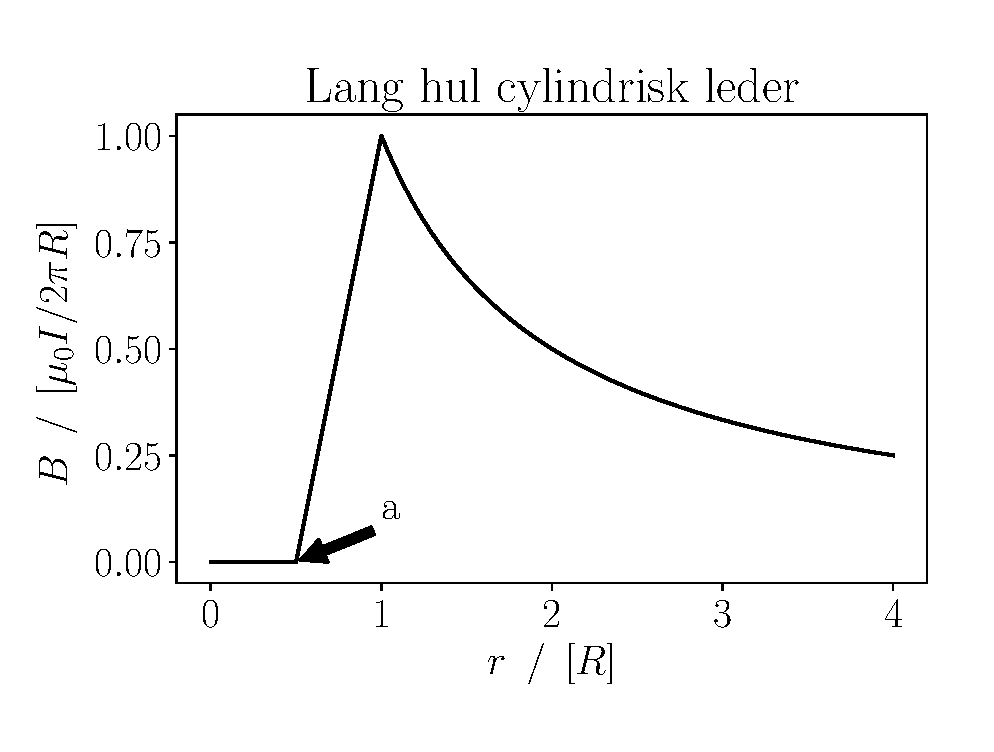
\includegraphics[width=\columnwidth]{facit/figurer/elektro/lange_lige_leder_hul_cylinder.eps}
            \caption{Hul cylindrisk leder med indre radius $a = R/2$ og ydre radius $R$.}
            \label{fig:lang_lige_hul_cylindrisk_leder}
        \end{subfigure}
        \caption{Størrelsen af af magnetfeltet for en lang lige leder med uniform strømfordeling som funktion af afstanden fra lederens centrum. Feltstyrken er angivet i enheder af den maksimale feltstyrke, $B(r/R)$.}
    \end{figure}
    %
    \opg Se figur \ref{fig:lang_lige_cylindrisk_leder}
    \opg Da cylinderen er hul med en indre radius $a$, løber der ingen strøm i området $r<a$. Ampereløkken kan vælges arbitræt indeni hulrummet uden at den vil indeslutte nogen strøm. For at opfylde Amperes lov må magnetfeltet derfor være nul i hulrummet og derfra har den samme form som for cylinderen uden hulrum, se figur \ref{fig:lang_lige_hul_cylindrisk_leder}.
\end{opgave}

\begin{opgave}{Eleveksperiment} \label{opg:EleveksperimentFacit}
    \opg Ligning \ref{eq:current} siger, at $I \equiv \dv{q}{t}$, og da vi må betragte $\dd{t}$ som en variabel, så må vi gange med den, så
    \begin{align} \label{eq:dq=Idt}
        \dd{q} = I \dd{t} \: .
    \end{align}
    \opg Vi kan nu integrere op ligning \ref{eq:dq=Idt}, hvor vi, når vi integrerer mht. $t$, integrerer fra $0$ til $T$ (det givne tidsrum), og integralet mht. $q$ integreres fra $q(t = 0)$ til $q(t = T)$. Vi får derved integralerne
    \begin{align}
        \int_0^T I(t) \, \dd{t} &= \int_{q(t = 0)}^{q(t = T)} \dd{q}
            = \left[q\right]_{q(t = 0)}^{q(t = T)}
            = q(t = T) - q(t = 0) \: .
    \end{align}
    \opg Idet strømmen først tændes til tiden $t = 0$, da vil der til $t=0$ ikke være nogen ladning:
    \begin{align}
        q(t = 0) &= 0 \: .
    \end{align}
    \opg Den totale ladning gennem amperemeteret efter et minut findes ved at indsætte $60$ sekunder (1 min) i stedet for $T$ i ligningen fra opgave \thechapter,\ref{opg:EleveksperimentFacit} delopgave 2, hvor $q(t = 0) &= 0$, så
    \begin{align}
        q(\SI{60}{\second}) &= \int_0^T I(t) \, \dd{t}
            = \int_{\SI{0}{\second}}^{\SI{60}{\second}} \frac{\SI{0,06}{\ampere\second}}{\SI{20}{\second} + t} \, \dd{t}
            = \left[\SI{0,06}{\ampere\second} \cdot \ln\left(\SI{20}{\second} + t\right)\right]_{\SI{0}{\second}}^{\SI{60}{\second}} \nonumber\\
            &= \SI{0,06}{\ampere\second}\left\{\ln\left(\SI{20}{\second} + \SI{60}{\second}\right) - \ln\left(\SI{20}{\second} + \SI{0}{\second}\right)\right\}
            = \SI{0,06}{\ampere\second}\left\{\ln\left(\SI{80}{\second}\right) - \ln\left(\SI{20}{\second}\right)\right\} \nonumber\\
            &= \SI{0,06}{\ampere\second} \cdot \ln\left(\frac{\SI{80}{\second}}{\SI{20}{\second}}\right)
            = \SI{0,06}{\ampere\second} \cdot \ln(4)
            = \SI{0,083}{\coulomb} \: .
    \end{align}
\end{opgave}

\begin{opgave}{Solenoiden}
    \opg Samme vej som indikeret på figur \ref{fig:solenoide_ampere}.
    \opg Linjestykket $cd$ er uendelig langt væk. Elektriske og magnetiske felter går, som tommelfingeregel, som $1/r^2$, hvilket betyder at de bliver mindre og mindre desto længere væk fra kilden man er. Er man uendelig langt væk, må feltet være uendelig småt, hvilket i fysikermatematik er det samme som 0.
    \opg Solenoiden er pr. antagelse meget lang ift. Ampereløkken. Feltlinjerne skal være kontinuerte og har form som en udstrukket ellipse, der indeslutter en del af solenoiden. Grundet solenoidens længde er ellipsen strukket så meget at den omkring midten af solenoiden er parallel med solenoiden -- dette gælder båden indenfor og udenfor solenoiden.
    \opg Af ovenstående er feltet vinkelret på, linjestykkerne $bc$ og $da$, hvorfor $\va B \cdot \dd{\va l} = 0$. For linjestykke $cd$ er feltet 0, hvorfor integralet også er, mens $\va B \cdot \dd{\va l} = B\dd{l}$ Ergo bliver det lukkede linjeintegral
    \begin{align*}
        \oint_P \va B \cdot \dd{l} = \int_{ab} B\dd{l} = B\int_0^L \dd{l} = BL.
    \end{align*}
    %
    \opg Den indesluttede strøm er antallet af ringe, som løkken indeslutter, $nL$, gange strømstyrken af strømmen i en enkelt leder, $I$. Ergo er
    \begin{align*}
        I_\mathrm{inde} = nLI.
    \end{align*}
    \opg Nu sættes informationerne ind i Amperes lov, ligning \eqref{eq:ampere}, hvor der fås
    \begin{align*}
        \oint_P \va B \cdot \dd{\va{l}} = \mu_0 I_\mathrm{inde} \implies BL = \mu_0nLI \implies B = \mu_0nI
    \end{align*}
    \opg Præcis i midten af solenoiden skal feltet være parallelt med solenoiden for at bevare den cylindriske symmetri. Tæt på midten er ellipserne så store, at der ikke er den store afvigelse fra de rette linjer, hvorfor feltet er nogenlunde uniformt
\end{opgave}


\subsection*{Induktion}

\begin{figure}
    \centering
    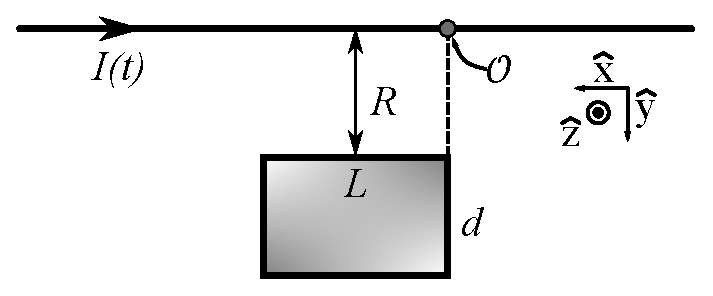
\includegraphics[width=.6\columnwidth]{facit/figurer/elektro/induktion_svar.eps}
    \caption{Skravering af det område løkken omkranser.}
    \label{fig:induktion_svar}
\end{figure}
%
\begin{opgave}{Induktion I}
    \opg Se figur \ref{fig:induktion_svar}.
    \opg Af argumenterne i afsnit \ref{sec:lang_lige_leder} er magnetfeltet fra en lang lige leder i et punkt kun afhængigt af afstanden fra lederen til punktet. I $xy$-planen er de beskrevet ved $y$-koordinatet, hvorfor magnetfeltet er uafhængigt af $x$- og $z$-koordinatet.
    \opg Fluxen gennem rektanglen er overfladeintegralet af magnetfeltet i det område. Hele rektanglen ligger i $xy$-planen, hvorfor dens arealelement er
    %
    \begin{align*}
        \dd{\va A} = \zhat\dd{x}\dd{y}.
    \end{align*}
    %
    Af højrehåndsreglen peger magnetfeltet ind i løkken og udskiftes $r$ med $y$ i ligning \eqref{eq:lang_lige_leder} er
    %
    \begin{align*}
        \va B = -\frac{\mu_0I(t)}{2\pi y}\zhat.
    \end{align*}
    %
    Koordinatsystemets nulpunkt vælges som vist på figur \ref{fig:induktion_svar}, og da $\zhat\cdot\zhat = 1$ bliver fluxen
    %
    \begin{align*}
        \Phi_B &= \int_R^{R+d} \int_0^L \va B \cdot \zhat \dd{x}\dd{y} = -\int_R^{R+d} \int_0^L \frac{\mu_0I(t)(t)}{2\pi y} \dd{x}\dd{y} = -\frac{\mu_0I(t)}{2\pi} \int_R^{R+d} y^{-1} \int_0^L \dd{x}\dd{y} \\
        &= -\frac{\mu_0I(t)}{2\pi} \int_R^{R+d} y^{-1} \Big[x\Big]_0^L \dd{y} = -\frac{\mu_0I(t)}{2\pi} \int_R^{R+d} y^{-1} L \dd{y} = -\frac{\mu_0LI(t)}{2\pi} \int_R^{R+d} y^{-1} \dd{y} \\
        &= -\frac{\mu_0LI(t)}{2\pi} \Big[\ln(y)\Big]_R^{R+d} = -\frac{\mu_0LI(t)}{2\pi} \Big[\ln(R+d) - \ln(R)\Big] = -\frac{\mu_0LI(t)}{2\pi}\ln\left(\frac{R+d}{R}\right).
    \end{align*}
    %
    \opg Først indsættes udtrykket for $I(t)$ i ovenstående flux og derefter bruges Faradays lov:
    %
    \begin{align*}
        \mathcal{E} &= -\dv{\Phi_B}{t} = \frac{\mu_0L}{2\pi}\ln\left(\frac{R+d}{R}\right)\dv{I(t)}{t} = \frac{\mu_0L}{2\pi}\ln\left(\frac{R+d}{R}\right)I_0\dv{}{t}\cos(\omega t) \\
        &= -\frac{\mu_0LI_0\omega}{2\pi}\ln\left(\frac{R+d}{R}\right)\sin(\omega t) = \frac{\mu_0LI_0\omega}{2\pi}\ln\left(\frac{R}{R+d}\right)\sin(\omega t).
    \end{align*}
    %
    \opg Af højrehåndsreglen peger magnetfeltet ind i eller ud af tegningen alt efter om $\cos(\omega t)$ er positiv eller negativ. Når $\sin(\omega t)>0$, så peger ændringen af feltet ind i tegningen og modsat, når $\sin(\omega t)<0$. Af Lenz' lov løber strømmen med uret, når $\sin(\omega t)>0$ og mod uret når $\sin(\omega t)<0$.
    \opg Den elektromotoriske kraft er et spændingsfald hvorfor
    %
    \begin{align}
        I = \frac{P}{\mathcal{E}} = \frac{2\pi P}{\mu_0LI_0\sin(\omega t)\ln\big[R/(R+d)\big]}.
    \end{align}
\end{opgave}

\begin{opgave}{Induktion II}
    \opg Definitionen af hastighed er den tidsafledede af sted, derfor er
    %
    \begin{align}
        \va v(t) = \dv{\va r(t)}{t} = \Big[at+v_0\Big]\xhat,
    \end{align}
    %
    hvilket det samme som i \eqref{eq:fart_induktion}.
    \opg Et arealelement består af en enhedsvektor og to infinitesimaler, hvor enhedsvektoren angiver planens normal. Af figur \ref{fig:induktion_ii} ligger opstillingen i $xy$-planen, hvorfor $\zhat$ er en på planen ortogonal enhedsvektor. Da opstillingen er i $xy$-planen skal infinitesimalerne være dem, der tilhører dette plan -- nemlig $\dd x$ og $\dd y$. Ergo er
    %
    \begin{align}
        \dd{\va a} = \zhat \dd{x}\dd{y}.
    \end{align}
    %
    \opg For at tilskrive koordinater til punkterne skal der vælges et nulpunkt. Det er smart at vælge et stillestående nulpunkt, og det er oftest lettest at arbejde med størrelser med positivt fortegn. Da $x$-aksen vokser mod højre og $y$-aksen vokser i opadgående retning er det smart at vælge et nulpunkt så alt foregår til højre for og over dette punkt. Det nederste venstre hjørne af rektanglet bevæger sig ikke, og alt er over og eller til højre for dette punkt, hvorfor det er et smart nulpunkt -- ergo er nederste venstre hjørne i $(0,0)$. Øverste venstre hjørne ligger på en lodret linje over det nederste venstre hjørne og afstanden imellem de to punkter er $L$. Derfor er øverste venstre hjørne i punktet $(0,L)$. Da lederen bevæger sig flytter dette punkt sig når tiden går, men det forbliver liggende på $x$-aksen. Det må have samme $x$-koordinat som selve lederen, hvorfor nederste venstre hjørne har koordinatet $\left(\va r(t),0\right)$. Tilsvarende må øverste højre hjørne have koordinatet $\left(\va r(t),L\right)$.
    \opg Definitionen af flux, ligning \eqref{eq:magnetisk_flux}, er et overflade integral, hvorfor der integreres over to variable. Der integreres over hele rektanglet og grænserne er defineret af rektanglets ydrepunkter. Fra de to forrige spørgsmål er fluxen derfor
    %
    \begin{align}
        \Phi_B = \int \va B \cdot \dd{\va a} = \int_{y_{min}}^{y_{max}} \int_{x_{min}}^{x_{max}} \va B \cdot \zhat \dd{x'}\dd{y} = \int_0^L \int_0^{x(t)} \va B \cdot \zhat \dd{x'}\dd{y}.
    \end{align}
    %
    Det er god skik at sætte mærker på de $x'er$ man integrerer over, da grænserne også inkluderer $x$. Man kan så ledes kende forskel på hvad der er integrationsvariablen og hvad der er grænserne. I dette tilfælde er det måske ikke svært, men ikke desto mindre er det en god vane.
    \opg Magnetfeltet er uniformt og derfor ikke stedsafhængigt og derudover peger det i negativ $z$-retning, hvorfor $\va B \cdot \zhat = -B_0$. Dette er en konstant, hvorfor den kan sættes udenfor begge integraler, der så reducerer til to integraler over en konstant:
    %
    \begin{align}
        \Phi_B &= -B_0\int_0^L \int_0^{x(t)} \dd{x'}\dd{y} = -B_0 \int_0^L \Big[x'\Big]_0^{x(t)} \dd{y} = -B_0 \int_0^L x(t) \dd{y} \nonumber \\
        &= -B_0x(t) \int_0^L \dd{y} = -B_0x(t) \Big[y\Big]_0^L = -B_0Lx(t) = -B_0L\left[\frac{1}{2}at^2 + v_0t + x_0\right].
    \end{align}
    %
    \opg Af Faradays lov, \eqref{eq:faraday}, er den elektromotoriske kraft i kredsløbet
    %
    \begin{align}
        \mathcal{E} &= -\dv{\Phi_B}{t} = -\dv{}{t}\left(-B_0L\left[\frac{1}{2}at^2 + v_0t + x_0\right]\right) \nonumber \\
        &= B_0L\left[\frac{1}{2}a\dv{}{t}t^2 + v_0\dv{}{t}t + \dv{}{t}x_0\right] = B_0L\Big[at + v_0\Big].
    \end{align}
    %
    \opg Først isoleres modstanden i formlen, $R = U^2/P$, og så indsættes den elektromotoriske kraft på spændingsforskellens plads
    %
    \begin{align}
        R = \frac{U^2}{R} \xrightarrow{\mathcal{E} \rightarrow U} \frac{1}{P}\left(B_0L\Big[at + v_0\Big]\right)^2 = \frac{(B_0L)^2}{P}\Big[at + v_0\Big]^2.
    \end{align}
    %
    \opg I første omgang er det en god idé at skrive udtrykket ud, så det er tydeligt hvilken funktionstype, der er tale om:
    %
    \begin{align}
        R = \frac{(B_0L)^2}{P}\Big[at + v_0\Big]^2 = \frac{(B_0L)^2}{P}\left[a^2t^2 + 2av_0t + v_0^2\right].
    \end{align}
    %
    Der er altså tale om et andengradspolynomium. Konstanterne er ikke vigtige, så derfor plottes $t,RP/(B_0L)$, da det gør det hele mere overskueligt. Dette er vist i figur \ref{fig:plot_induktion_ii}.
    \opg Her stoppes tallene blot ind i formlen fra spørgsmål 7), \eqref{eq:induktion_ii_modstand}, som efter en smule enhedsomregning til SI-enheder giver resultatet
    %
    \begin{align}
        R = \SI{15,6}{\ohm}.
    \end{align}
\end{opgave}

\begin{figure}
    \centering
    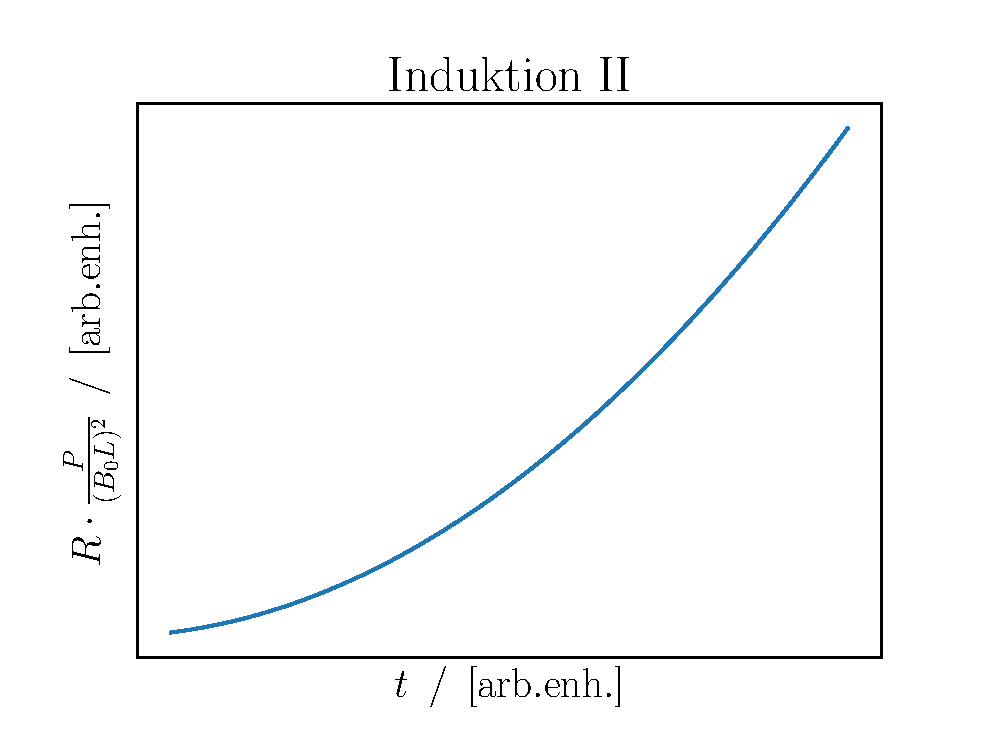
\includegraphics[width=.6\columnwidth]{facit/figurer/opg_induktion_ii.eps}
    \caption{Plot af modstanden i elpæren som funktion af tid. Bemærk akserne, der er plottet i arbitrære enheder og med konstanterne langt ind i selve 2. aksen, som konventionen i teoretisk fysik foreskriver.}
    \label{fig:plot_induktion_ii}
\end{figure}